\section{Архитектура и проектирование приложения}
\label{sec:arch_and_mod}
 
\subsection{Android}
Так как для разработки был выбран Android SDK, то при разработке было решено придерживаться характерных для данной платформы архитектурных подходов.
На данный момент стандартом в Android разработке является MVVM \cite{web7}.
Она заключается в отделении пользовательского интерфейса от логики приложения. Опишем каждый компонент данного архитектурного подхода (cхема на рисунке~\ref{fig:arch:docs_connections}).

Model~-- слой с основной логикой программы.
View~-- пользовательский интерфейс.
ViewModel~-- связывающая прослойка между View и Model.

\begin{figure}[H]
 \centering
   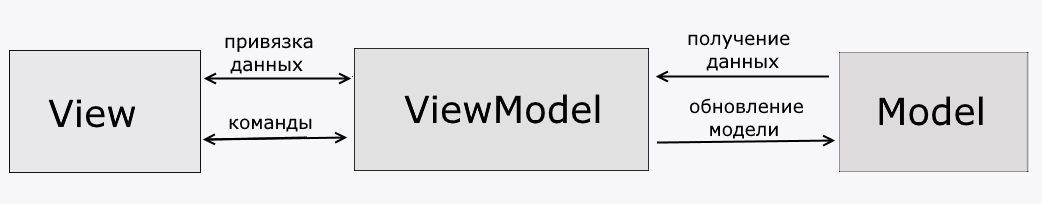
\includegraphics[scale=0.3]{mvvm.png} 
   \caption{MVVM}
   \label{fig:arch:docs_connections}
\end{figure}

Для упрощения реализации части проектирования и упрощения разработки, компания Google выпустила Android Architecture Components \cite{web8}. Данный набор решений включает в себя:

\begin{itemize}
 \item Lifecycle~-- отслеживает текущий статус Activity и может уведомлять об этом своих подписчиков;
 \item LiveData~-- получает и хранит данные, может отправлять их своим подписчикам;
 \item ViewModel~-- поможет сохранить живыми необходимые для вас объекты при повороте экрана;
 \item Paging Library~-- библиотека для постраничной загрузки данных из базы данных, с сервера или любого другого источника;
 \item Navigation Architecture Component~-- новый компонент для навигации по экранам приложения;
 \item Work Manager~-- удобный механизм выполнения фоновых задач;
 \item Room~-- обёртка для работы с базой данных;
 \item Data Binding~-- избавление от рутины по написанию кода работающего со View;
 \item Coroutines~-- потоки исполнения кода, которые организуются поверх аппаратных потоков.
 \end{itemize}

 Основные плюсы MVVM включают в себя:

\begin{itemize}
  \item лёгкость в тестировании (связи между логикой приложения и пользовательским интерфейсом ослабевает, что даёт большую гибкость в тестировании отдельных компонентов);
  \item прост в поддержке (высокая модульность и прозрачность слоёв архитектуры приносят простоту в отслеживании ошибок и расширении приложения);
  \item прозрачная комьюникация (ViewModel предоставляют простой интерфейс, который View использует для заполнения себя, сама же ViewModel связывает View с частью бизнес-логики приложения).
\end{itemize}
 
\subsection{Serverless архитектура}
Serverless-вычисления (бессерверные-вычисления) - модель облачных вычислений, в которых платформа динамически руководит выделением вычислительных ресурсов. 
В данном случае бессерверный не означает отсутствие сервера как такового, под этим понимается то, что пользователю конкретной платформы не нужно заниматься созданием и настройкой собственного сервера. 
Данный подход позволяет значительно сэкономить ресурсы и уменьшить срок разработки, так как многие важные аспекты серверной части на себе берёт платформа. 
В рамках данного проекта такой платформой выступает Firebase.
 
\subsection{Организация и описание модулей приложения}
Разработанное мобильное приложение можно разделить на три составляющие:
\begin{itemize}
 \item клиентское приложения на Kotlin;
 \item модуль Firebase для работы с базой данных;
 \item API cервер для получения данных.
\end{itemize}
 
Клиентское приложение является основным модулем для данного проекта. В рамках клиентского приложения реализованы основные функциональные возможности данного проекта:
\begin{itemize}
  \item поддержка множества магазинов;
  \item возможность фильтровать поиск по множеству фильтров;
  \item вкладка избранное, возможность добавлять игры или предложения в избранное;
  \item вкладка исследование, главная вкладка с предложениями которые ранжирует само приложение;
  \item просмотр дополнительной информации (рейтинг, самая высокая стоимость, самая низкая стоимость и тд);
  \item возможность перехода на сторонние магазины для покупки товара;
  \item социальные функции (шейринг, отображение графики, ведение статистики пользователя).
\end{itemize}
 
Модуль Firebase отвечает за авторизацию, управление данными пользователя, их организацию и процесс передачи данных клиентскому приложению.
 
API сервер представлет собой несколько сторонних бесплатных API серверов с базами данных игр и игровых магазинов. Основная функция этих серверов заключается в выдаче клиенту необходимой для работы информации (список магазинов, дополнительная информация об игре, поиск лучший предложений), а также объединении нескольких сторонних API в единое целое на клиентской части.
 
На рисунке~\ref{fig:arch:modules_scheme} изображена схема взаимодействия вышеперечисленных модулей.
 
\begin{figure}[H]
 \centering
   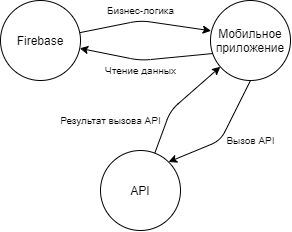
\includegraphics[scale=0.8]{api.png} 
   \caption{Структура модулей приложения}
   \label{fig:arch:modules_scheme}
\end{figure}
 
\section{Реализация мобильного приложения}
\label{sec:code}
По итогу разработки было реализовано мобильное приложение, которое позволяет пользователю находить лучшие предложения по продаже игр среди игровых магазинов.

\subsection{Базовые компоненты}

Для удобной и расширяемой архитектуры приложения были написаны базовые компоненты для Activity, Fragment, ViewModel. Рассмотрим каждый в отдельности.

\undersection{BaseActivity}~\par
Activity представляет собой отдельный модуль приложения с которым пользователь может взаимодействовать. Для удобства был написан базовый класс (см. листинг~\ref{lst:add:a_1}), который реализует обработку ошибок путем вызова диалогового окна с текстом ошибки, а также показом прогресса загрузки данных с сервера дополнительно с блокированием интерфейса пользователя, пока запрос на сервер не будет выполнен. Помимо блокирования пользовательского интерфейса данная реализация решает проблему синхронизации при нескольких запросах на сервер путем @Synchronized аннотаций и проверок на существования прогресса на экране. Аннотация @Synchronized позволяет быть уверенным в том, что в данный метод заходит только 1 поток, при том, что для остальных потоков данный метод не будет доступен, пока первый поток не завершит свои задачи. Данный класс является базовым для любой Activity в приложении.
\undersection{BaseFragment}~\par
Fragment является модульной переиспользуемой частью Activity. Класс BaseFragment (см. листинг~\ref{lst:add:a_2}) является базовым классом для всех фрагментов в приложении. Данный класс реализует передачу событий загрузки в Activity, а также логику по работе с клавиатурой и проверке доступов к различным подсистемам Android. Также данный класс обязывает реализовывать для каждого фрагмента базовую ViewModel.

\undersection{BaseViewModel}~\par
ViewModel~-- модель представления, которая служит прослойкой между View и Model. Такое разделение позволяет ускорить разработку и поддерживаемость программы~-- можно менять один компонент, не затрагивая код другого. Данная реализация базовой ViewModel (см. листинг~\ref{lst:add:a_3}) включает в себя определение событий ошибок, загрузок, а также вспомогательных методов для запросов в сеть.

\subsection{Слой данных и логики}
Всю бизнес-логику и логику работы с получением данных можно представить в виде дерева зависимостей, состоящего из:

\begin{itemize}
  \item слой Api для запросов на сервера;
  \item слой Database для работы с локальной базой данных;
  \item слой DataSource для получения данных либо из Api, либо из Database;
  \item слой Gateway для преобразования данных в модели приемлимые для приложения;
  \item слой UseCase для инкапсулирования логики Gateway и другой бизнес-логики.
\end{itemize}

На рисунке~\ref{fig:arch:data_diagram} изображена схема взаимодействия вышеперечисленных модулей.
 
\begin{figure}[H]
 \centering
   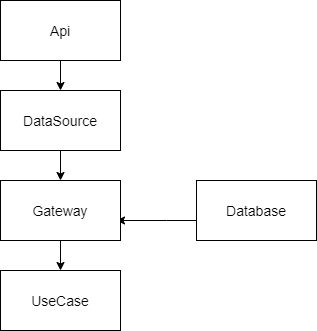
\includegraphics[scale=0.8]{data_diagram.png} 
   \caption{Структура слоя данных}
   \label{fig:arch:data_diagram}
\end{figure}
 
В качестве примера рассмотрим получение списка магазинов в приложении. Интерфейс вызывает UseCase GetStores (см. листинг~\ref{lst:getStores}).

\begin{lstlisting}[language=Java,label={lst:getStores},caption={UseCase GetStores}]
class GetStores(private val storesGateway: StoresGateway) {
    suspend operator fun invoke(): List<Store> {
        return storesGateway.getStores()
    }
}
\end{lstlisting}

Данный UseCase вызывает StoresGateway (см. листинг~\ref{lst:storesGateway}), который осуществляет получение магазинов либо из базы данных, либо с сервера, попутно сохраняя их в базу данных. Данный метод проверяет наличие интернет подключение на устройстве, после этого делает запрос на сервер, либо в локальную базу данных, в зависимости от результата. Также выполняются преобразования моделей в модели подходящие приложению. Если интернет подключение на устройстве присутствует и получение списка магазинов с сервера произошло успешно, то метод сохраняет полученные магазины в локальную базу данных для дальнейшего использования.
\begin{lstlisting}[language=Java,label={lst:storesGateway},caption={StoresGateway}]
class StoresGatewayImpl(
    private val storesDataSource: StoresDataSource,
    private val storesDao: StoreLocalDao,
    private val networkService: NetworkService
) : StoresGateway {
    override suspend fun getStores(cachedFirst: Boolean): List<Store> {
        val stores = storesDao.getStores()
        if ((cachedFirst && stores.count() > 0) || !networkService.isNetworkEnabled) {
            return storesDao.getStores().map { it.toDomain() }
        } else if (networkService.isNetworkEnabled) {
            val storesRemote = storesDataSource.getStores().map {
                Store(
                    it.storeID, it.storeName, it.isActive != 0,
                    StoreImage(
                        Uri.parse("${Constants.HOST_URL}${it.storeImage.bannerPath}"),
                        Uri.parse("${Constants.HOST_URL}${it.storeImage.logoPath}"),
                        Uri.parse("${Constants.HOST_URL}${it.storeImage.iconPath}")
                    )
                )
            }
            val storesDB = storesDao.getStores()
            storesRemote.forEach { storeItem ->
                val store = storesDB.findLast { item -> item.storeID == storeItem.id }
                if (store != null) {
                    storeItem.isSelected = store.isSelected
                }
            }
            storesDao.replaceStores(storesRemote.map { obj -> obj.toDb() })
            return storesRemote
        }
        return arrayListOf()
    }
}

\end{lstlisting}


StoresGateway применяет один из двух источников данных. При наличии подключения к интернету вызывается StoresDataSource(см. листинг~\ref{lst:storesDataSource}), который делает запрос на сервер.

\begin{lstlisting}[language=Java,label={lst:storesDataSource},caption={StoresDataSource}]
class StoresDataSource(private val api: Api) {
    suspend fun getStores(): List<StoreRemote> {
        return api.getStores()
    }
}
\end{lstlisting}

Интерфейс Api (см. листинг~\ref{lst:storesApi}) реализуется с помощью библиотеки Retrofit, которая является одной из самых популярных и удобных библиотек для запросов на сервер на устройствах Android.

\begin{lstlisting}[language=Java,label={lst:storesApi},caption={Api}]
interface Api {
    @GET("stores")
    suspend fun getStores(): List<StoreRemote>
}
\end{lstlisting}

Если же интернет подключение отсутствует, то вызывается объект класса под названием StoresLocalDao (см. листинг~\ref{lst:storesLocalDao}), которое инкапсулирует логику для работы с локальной базой данных.
\begin{lstlisting}[language=Java,label={lst:storesLocalDao},caption={StoresLocalDao}]
@Dao
abstract class StoreLocalDao : BaseDao<StoreLocal> {
    @Query("SELECT * FROM stores")
    abstract suspend fun getStores(): List<StoreLocal>

    @Query("DELETE FROM stores")
    abstract suspend fun clearStores()

    @Transaction
    open suspend fun replaceStores(objects: List<StoreLocal>) {
        clearStores()
        insert(objects)
    }
}
\end{lstlisting}

\subsection{Внедрение зависимостей}
Внедрение зависимости~-- процесс предоставления внешней зависимости программному компоненту. Является специфичной формой инверсии управления, когда она применяется к управлению зависимостями. В полном соответствии с принципом единственной обязанности объект отдаёт заботу о построении требуемых ему зависимостей внешнему, специально предназначенному для этого общему механизму. Для внедрения зависимостей в работе используется легковесная библиотека Koin. Концепция области в Koin аналогична таковой в Android. Она позволяет, например, ограничить область живучести модели представления (ViewModel) до определенной активности и использовать эту модель во фрагментах, которыми наполняется активность. Как правило, в Koin три вида временных областей:

\begin{itemize}
  \item single, создается объект, который сохраняется в течение всего периода существования контейнера;
  \item factory, каждый раз создается новый объект, без сохранения в контейнере;
  \item scoped, создается объект, который сохраняется в рамках периода существования связанной временной области.
\end{itemize}

Для определения зависимостей в приложении используются следующие модули:
\begin{itemize}
  \item модуль Main, который определяет общие для всего приложения зависимости, как Api, базу данных, парсеры;
  \item модуль Database определяет источники данных для доступа к базе данных;
  \item модуль Service определяет вспомогательные сервисы для приложения;
  \item модуль DataSource определяет источники данных;
  \item модуль Gateway;
  \item модуль UseCase;
  \item модуль ViewModel.
\end{itemize}


В качестве примера приведён модуль Gateway (см. листинг~\ref{lst:add:a_4}), определяющий все классы Gateway в приложении.

\subsection{Манифест приложения}
Файл манифеста AndroidManifest.xml (см. листинг~\ref{lst:add:a_5}) предоставляет основную информацию о программе системе. Каждое приложение должно иметь свой файл AndroidManifest.xml. Файл манифеста инкапсулирует всю архитектуру Android-приложения, его функциональные возможности и конфигурацию. Корневым элементом манифеста является <manifest>. Обязательными являются элементы <application> и <uses-sdk>. Основной элемент манифеста <application> содержит множество дочерних элементов, определяющих структуру и работу приложения. Порядок расположения элементов, находящихся на одном уровне, произвольный. Все значения устанавливаются через атрибуты элементов. Кроме обязательных элементов, упомянутых выше, в манифесте по мере необходимости используются другие элементы.

\undersection{AhriMessagingService}~\par

Сервис который используется для получения и отображения нотификаций полученных через Firebase Cloud Messaging. Конкретной реализации данный сервис не имеет (см. листинг~\ref{lst:firebase_notifications}) и инкапсулирует базовую логику отображения нотификаций пользователю когда приложение выключено.

\begin{lstlisting}[language=Java,label={lst:firebase_notifications},caption={AhriMessagingService}]
class AhriMessagingService: FirebaseMessagingService() {

    override fun onMessageReceived(p0: RemoteMessage) {
        super.onMessageReceived(p0)
    }

    override fun onNewToken(p0: String) {
        super.onNewToken(p0)
    }
}
\end{lstlisting}

\undersection{HistoryProvider}~\par
Поставщик содержимого~-- это оболочка, в которую заключены данные. Если приложение использует базу данных SQLite, то только приложение имеет к ней доступ. Но бывают ситуации, когда данные желательно сделать общими. Простой пример~-- контакты из телефонной книги тоже содержатся в базе данных, но приложению нужно иметь доступ к данным, чтобы приложение тоже могло выводить список контактов. Так как исходное приложение не имеет доступа к базе данных чужого приложения, был придуман специальный механизм, позволяющий делиться своими данными всем желающим. Каждый поставщик содержимого регистрируется в устройстве как веб-сайт, при помощи специальной строки (она похожа на доменное имя и называется authority). Такая уникальная последовательность набора символов в устройстве представляет собой основу для набора ссылки для доступа к данным.

Данный поставщик содержимого не имеет конкретной реализации и используется для сохранения поисковых запросов пользователя. Данный поставщик включает в себя функционал удаления, добавления и обновления поисковых запросов.

\undersection{FileProvider}~\par
FileProvider является поставщиком содержимого который используется для доступа ко внутренним файлам приложения во время того как пользователь меняет свой аватар. Пример использования приведён ниже (см. листинг~\ref{lst:file_provider}).

\begin{lstlisting}[language=Java,label={lst:file_provider},caption={Использование FileProvider}]
    private fun getOutputMediaFile(name: String): Uri {
        val directory = requireActivity().applicationContext.getExternalFilesDir(null)
            ?: requireActivity().applicationContext.filesDir
        !directory.exists() && directory.mkdirs()

        return FileProvider.getUriForFile(
            requireActivity(),
            requireActivity().applicationContext.packageName + ".fileprovider",
            File(directory.path, name)
        )
    }
\end{lstlisting}

\subsection{Основные модули}

Приложение состоит из 7 взаимосвязанных модулей. Пользователь начинает знакомство с приложением с модуля приветствия после переходя в модуль авторизации, где ему будет необходимо зарегистрироваться в системе, после данных действий пользователь сможет взаимодействовать с основными модулями:

\begin{itemize}
  \item модуль исследования;
  \item модуль избранного;
  \item модуль поиска;
  \item модуль магазинов;
  \item модуль аккаунта.
\end{itemize}

\undersection{Модуль приветствия}~\par
Данный модуль создан для описания пользователю основных функций приложения. Модуль состоит из одной OnboardingActivity, которая в себя включает постраничное отображение преимуществ приложения. Пользователь может пропустить часть приветствия нажав кнопку SKIP и подтвердив свой выбор в диалоге. Пример пользовательского интерфейса представлен на рисунке~\ref{fig:arch:onboarding_1}.

\begin{figure}[H]
 \centering
   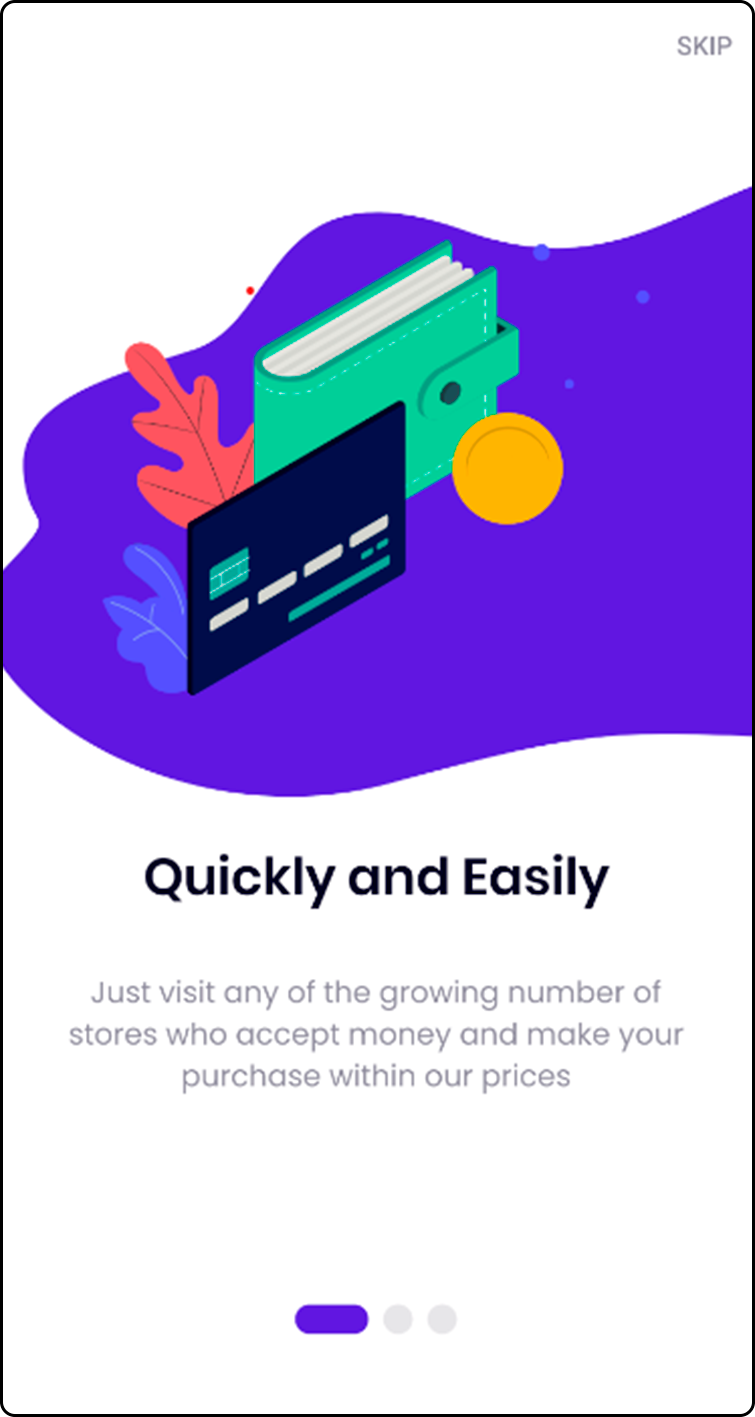
\includegraphics[scale=0.25]{onboarding_1.png} 
   \caption{Модуль приветствия}
   \label{fig:arch:onboarding_1}
\end{figure}

Программная реализация включает OnboardingFragmentStateAdapter, который использует отдельный Fragment для каждой из страниц описания (см. листинг~\ref{lst:onboarding_code}). При постраничном перелистывании данный адаптер вызывает отдельный Fragment с описанием конкретной функции используя позицию для обозначения нужного фрагмента.


\begin{lstlisting}[language=Java,label={lst:onboarding_code},caption={OnboardingFragmentStateAdapter}]
class OnboardingFragmentStateAdapter(activity: FragmentActivity) : FragmentStateAdapter(activity) {
    override fun createFragment(position: Int): Fragment {
        return when (position) {
            OnboardingStep.STEP_1.ordinal -> OnboardingStep1Fragment()
            OnboardingStep.STEP_2.ordinal -> OnboardingStep2Fragment()
            OnboardingStep.STEP_3.ordinal -> OnboardingStep3Fragment()
            else -> {
                throw Exception("Wrong Implementation")
            }
        }
    }
}
\end{lstlisting}


При долистывании до конца или подтверждения пропуска приветствия приложение вызывает функцию launchMain (см. листинг~\ref{lst:launch_main}), которая проверяет аутентифицирован ли пользователь. В зависимости от результата пользователь попадает на модуль авторизации, либо в главную часть приложения. Для запуска новых Activity, в приложении используются намерения.

Намерение~-- это механизм для описания одной операции~-- выбрать фотографию, отправить письмо, сделать звонок, запустить браузер и перейти по указанному адресу. В Android-приложениях многие операции работают через намерения. Но это не единственный вариант использования намерения. Также можно использовать для объявления о запуске активности или сервиса, направленных на выполнение каких-либо действий (как правило, речь о работе с определенной частью данных) или для передачи уведомлений о том, что произошло некое событие (или действие). Android транслирует намерения для объявления о системных событиях, например об изменениях в состоянии сетевого подключения или в уровне заряда батареи. Системные приложения в Android, такие как программы дозвона, регистрируют компоненты, отслеживающие заданные намерения, например входящий звонок или получено новое сообщение, и соответствующим образом реагируют на них.

\begin{lstlisting}[language=Java,label={lst:launch_main},caption={Функция launchMain}]
    private fun launchMain() {
        viewModel.isOnboardingEnabled = false
        val intent = if (isLoggedIn()) {
            Intent(applicationContext, MainActivity::class.java)
        } else {
            Intent(applicationContext, AuthActivity::class.java)
        }
        startActivity(intent)
        finish()
    }
\end{lstlisting}


\undersection{Модуль авторизации}~\par

Модуль авторизации состоит из одной AuthActivity, а также нескольких фрагментов между которыми происходит навигация внутри этой Activity.

AuthStartFragment является стартовым фрагментом в AuthActivity, он позволяет совершить навигацию на фрагмент логина AuthSignInFragment или на фрагмент регистрации пользователя AuthSignUpFragment.

AuthSignInFragment выполняет функцию аутентификации пользователя с помощью email и пароля, также имея возможность перейти на экран восстановления пароля или на экран регистрации пользователя. Пример пользовательского интерфейса представлен на рисунке~\ref{fig:arch:auth_2}.

\begin{figure}[H]
 \centering
   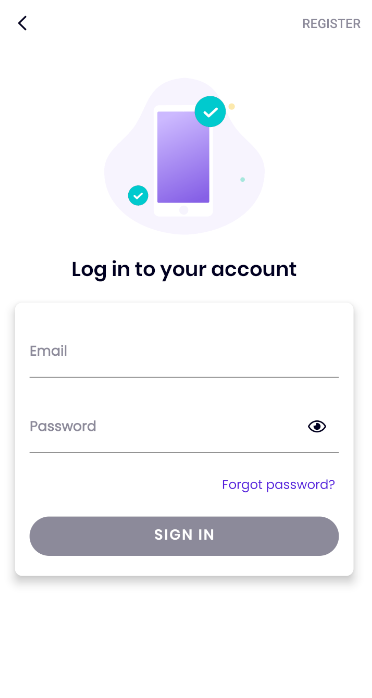
\includegraphics[scale=0.25]{auth_2.png} 
   \caption{Фрагмент аутентификации пользователя}
   \label{fig:arch:auth_2}
\end{figure}

Программная реализация содержит AuthSignInViewModel, который проводит базовую валидацию полей email и пароля с помощью ValidateEmail и ValidatePassword (см. листинг~\ref{lst:add:a_6}).

При нажатии на кнопку Sign In клиентское приложение делает запрос на Firebase Auth с помощью logIn метода (см. листинг~\ref{lst:auth_sign_in_uc}), который проверяет правильность введенных данных и делает запрос на сервер с этими данными. При неправильно введенных данных пользователь получает оповещение в виде сообщения на экране, что нужно ввести правильные данные.

\begin{lstlisting}[language=Java,label={lst:auth_sign_in_uc},caption={SignIn}]
    override suspend fun signIn(email: String, password: String) {
        return suspendCoroutine { cont ->
            auth.signInWithEmailAndPassword(email, password).addOnCompleteListener {
                    if (it.isSuccessful) { cont.resume(Unit) }
                     else { cont.resumeWithException(Exception("Wrong login or password")) }
              }}
    }
\end{lstlisting}

AuthSignUpFragment производит регистрацию пользователя с помощью email, пароля и имени пользователя, также имея возможность перейти на AuthSignInFragment. Пример пользовательского интерфейса представлен на рисунке~\ref{fig:arch:auth_3}.

\begin{figure}[H]
 \centering
   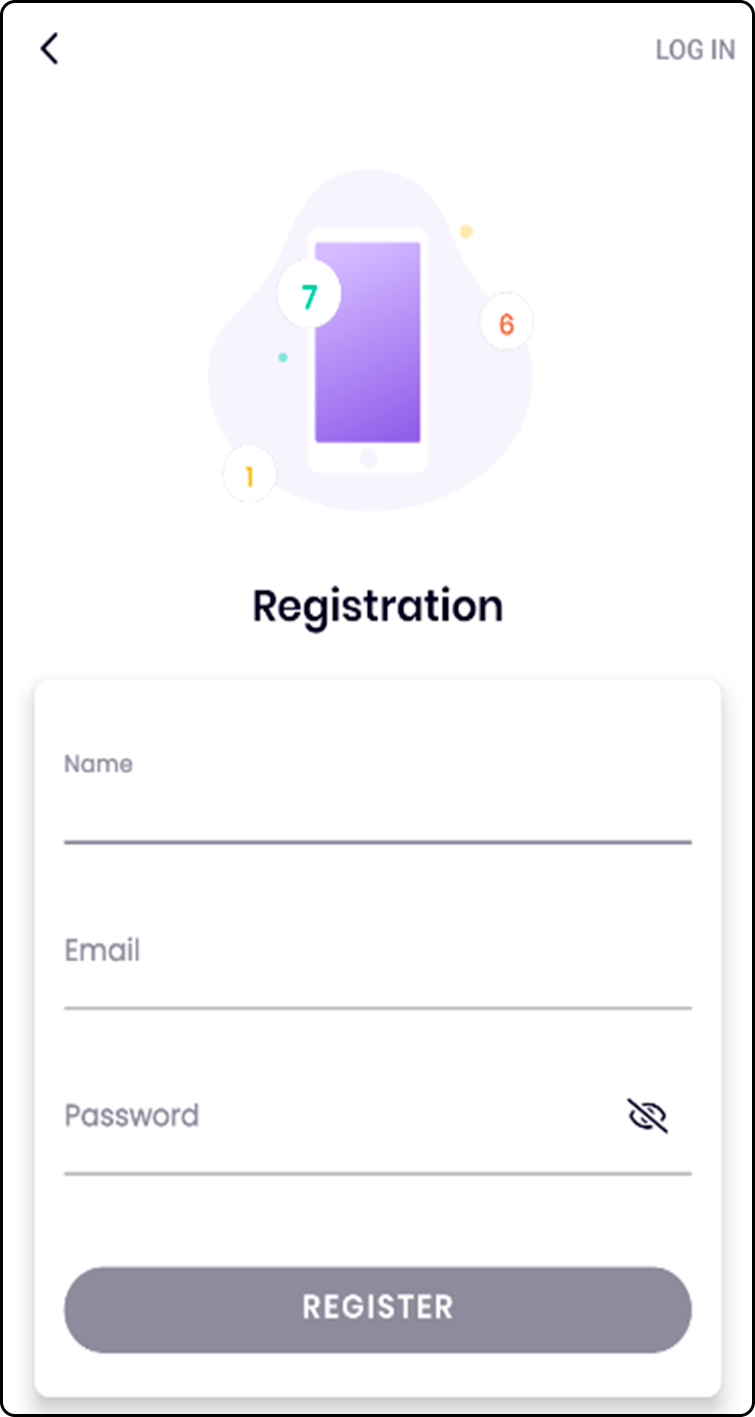
\includegraphics[scale=0.25]{auth_3.png} 
   \caption{Фрагмент регистрации пользователя}
   \label{fig:arch:auth_3}
\end{figure}

Пользователь нажимая на кнопку Register вызывает метод register, который производит базовую валидацию полей и делает запрос на регистрацию пользователя в Firebase Auth (см. листинг~\ref{lst:auth_sign_up_uc}).
\begin{lstlisting}[language=Java,label={lst:auth_sign_up_uc},caption={SignUp}]
auth.createUserWithEmailAndPassword(email, password).addOnCompleteListener {
                    if (it.isSuccessful) { auth.currentUser?.updateProfile(
                            UserProfileChangeRequest.Builder().setDisplayName(name).build())
                        cont.resume(Unit) } else {
                        cont.resumeWithException(Exception(if (it.exception != null) it.exception!!.message else "Wrong login or password"))
                    }
                }
\end{lstlisting}

Стоит заметить, что данный метод инкапсулирует в себе еще один запрос на изменения профиля пользователя, так как изначально регистрация проходит только с полями email и пароля, поэтому требуется дополнительный запрос на смену профиля при завершении регистрации.

\undersection{Модуль исследования}~\par
Модуль исследования позволяет пользователю просмотреть самые интересные новинки и новости из мира игр за последнее время. Модуль состоит из ExploreFragment, который является основным фрагментом в данном модуле и StoryFragment, показывающий истории наподобии Instagram. Примеры пользовательского интерфейса представлены на рисунках~\ref{fig:arch:explore_1} и ~\ref{fig:arch:explore_2}.

\begin{figure}[H]
 \centering
   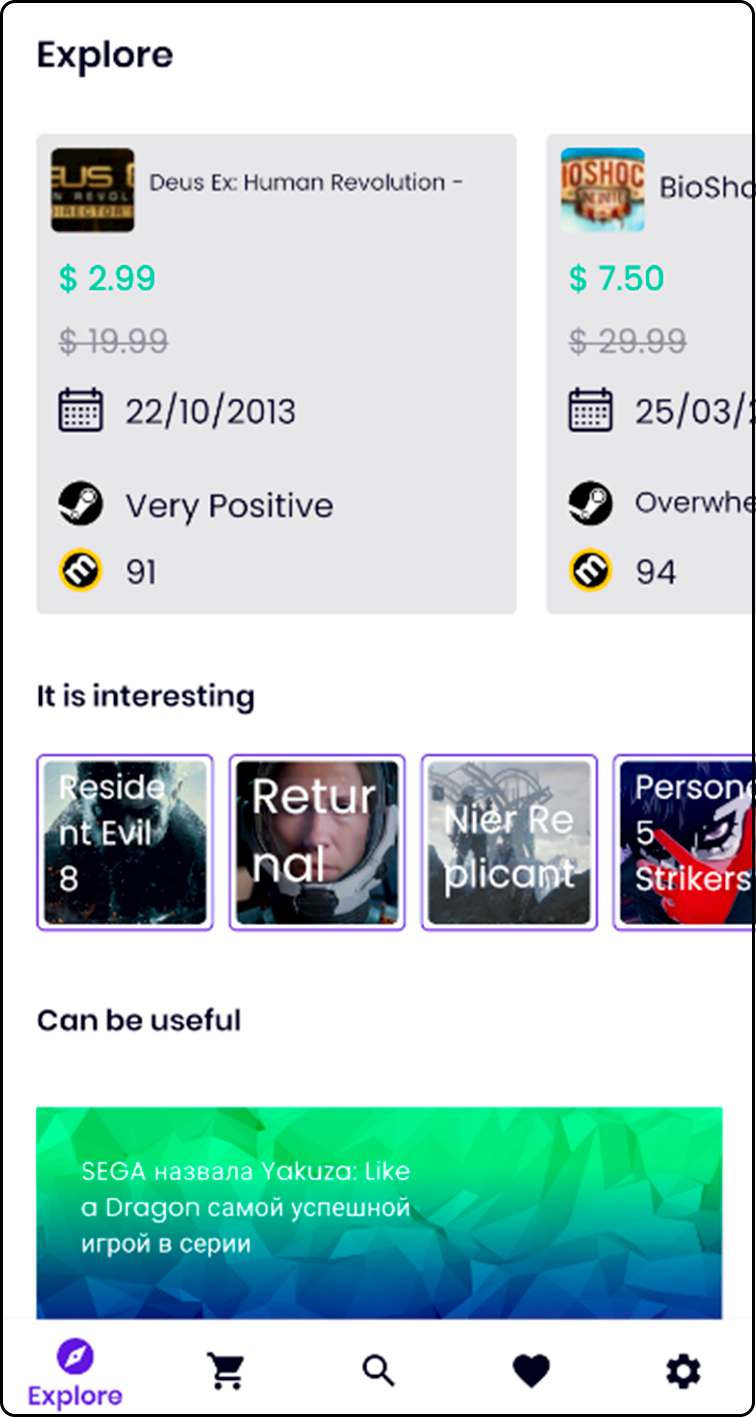
\includegraphics[scale=0.25]{explore_1.png} 
   \caption{ExploreFragment}
   \label{fig:arch:explore_1}
\end{figure}

\begin{figure}[H]
 \centering
   
\includegraphics[scale=0.25]{explore_2.png} 
   \caption{ExploreFragment}
   \label{fig:arch:explore_2}
\end{figure}

Экран исследования состоит из трёх блоков:

\begin{itemize}
  \item список игр проходящий ранжирование через фильтр рейтинга, отображаются игры с рейтингом выше 90 по Metacritic;
  \item список историй с последними новинками, позволяющий изучить как выглядит игра и перейти по ссылке для поления большей информации;
  \item колонка статей с посленими новостями из мира игр.
\end{itemize}

Список игр релизован через постраничное получение игр с сервера для оптимизации интерфейса. Когда пользователь долистывает до конца списка, то приложение делает запрос на следующую страницу игр и отображает её в исходном списке. Основным моментом в программной реализации является DealsPagingSource (см. листинг~\ref{lst:add:a_10}), который выполняет подсчет страниц и обработку ошибок для каждой отдельной страницы.

Истории реализованы наподобии Instagram, при нажатии на отдельную историю открывается отдельный фрагмент StoryFragment. Программная реализация включает в себя обработку жестов нажатий для переключения историй вперед и назад, данная логика реализуется с помощью класса GestureDetectorCompat (см. листинг~\ref{lst:add:a_7}). По нажатию на экран данный класс получает координаты нажатия, после этого происходит сравнение с шириной экрана, после данного действия алгоритм решает пролистать назад истории или вперед.

Блок последних новостей выполнен в виде вертикального списка с переходом на статью по нажатию на отдельный элемент списка. Получение списка новостей происходит с помощью запроса на отдельный сервер, где хранятся все последние новости игровой индустрии. Данные лежат в формате XML, соответственно преобразование данных происходит из этого формата с помощью SimpleXmlConverter из библиотеки Retrofit. Данный формат требует отдельной обработки в доменных классах приложения, рассмотрим класс RssChannel (см. листинг~\ref{lst:explore_rss}). В данном классе используются аннотации @Root, @Element, @ElementList, что соответствуют отдельным элементам целевого XML файла и позволяет XML преобразователю правильно обрабатывать файлы и переносить их в доменную область приложения. 

\begin{lstlisting}[language=Java,label={lst:explore_rss},caption={RssChannel}]
@Root(name = "channel", strict = false)
public class RssChannel
{
    @Element
    private String title;

    @Element
    private RssImage image;

    @ElementList(inline = true, required = false)
    public List<RssItem> item;

    @Override
    public String toString() {
        return "Channel [image=" + image + ", item=" + item + "]";
    }
}
\end{lstlisting}

\undersection{Модуль избранного}~\par
Экран избранного состоит из двух вкладок Deals и Games. Данные вкладки показывают все понравившиеся пользователю предложения по играм и сами игры. Добавление в избранное реализовано сохранением в локальную базу данных необходимых для отображения полей с идентификатором пользователя который добавил эти предложения в избранное. Пример пользовательского интерфейса представлен на рисунке~\ref{fig:arch:favorites_1}.

\begin{figure}[H]
 \centering
   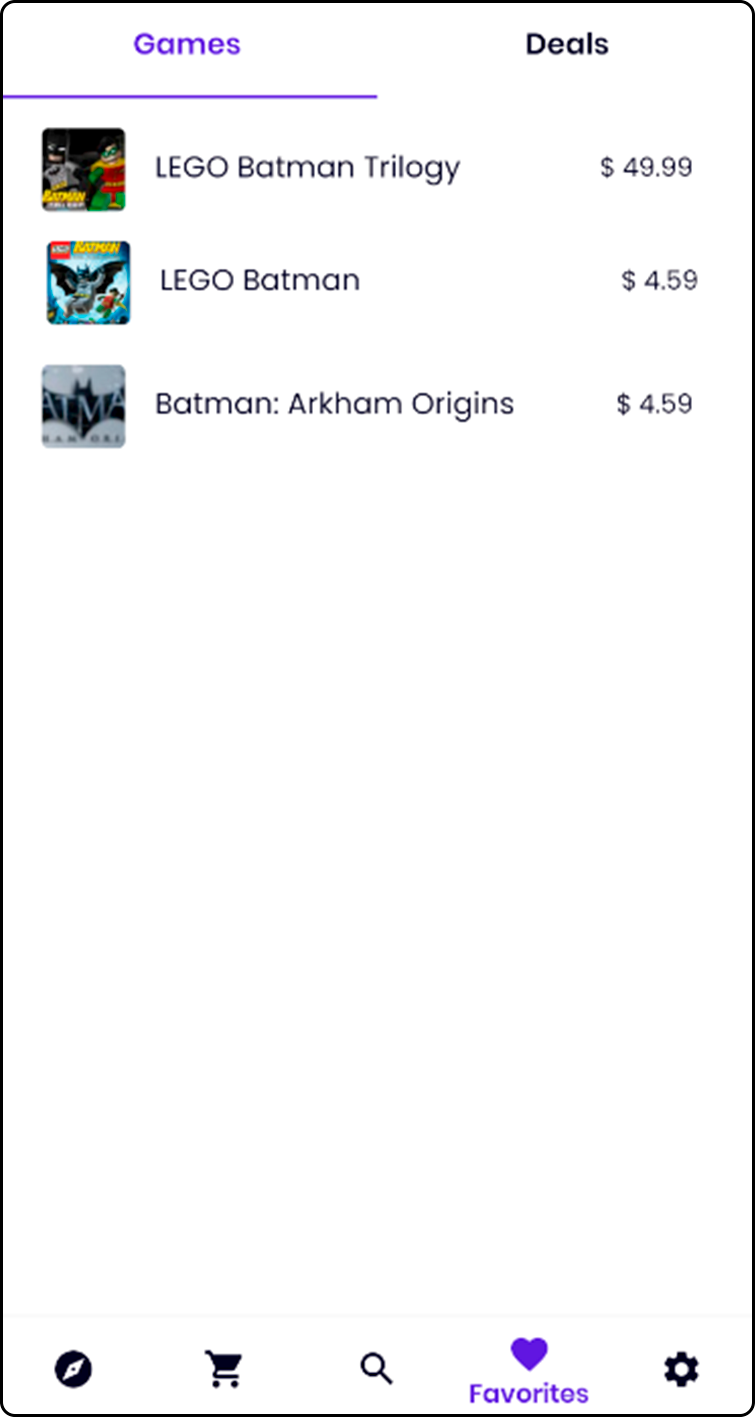
\includegraphics[scale=0.25]{favorites_1.png} 
   \caption{FavoritesFragment}
   \label{fig:arch:favorites_1}
\end{figure}

Помимо списков, в реализации присутствуют отдельные методы для загрузки картинок с помощью библиотеки Glide. В работе написано множество методов для их загрузки с множеством опций в классе UriBindingAdapter (см. листинг~\ref{lst:add:a_8}). Класс реализует одну из функций основных библиотек Android - DataBinding. Данная функциональность позволяет использовать методы прямо в коде интерфейса XML, что является удобным сокращением и повышает переиспользуемость методов.

При нажатии на сохраненную игру открывается соответствующий экран с информацией об этом предложении. Пример пользовательского интерфейса представлен на рисунке~\ref{fig:arch:favorites_3}. Данный экран включает в себя название, возможность добавить и удалить из избранного, лучшую цену за все времена, ссылку на Steam и Metacritic, а также список магазинов в которых эту игру можно купить и по каким ценам.

\begin{figure}[H]
 \centering
   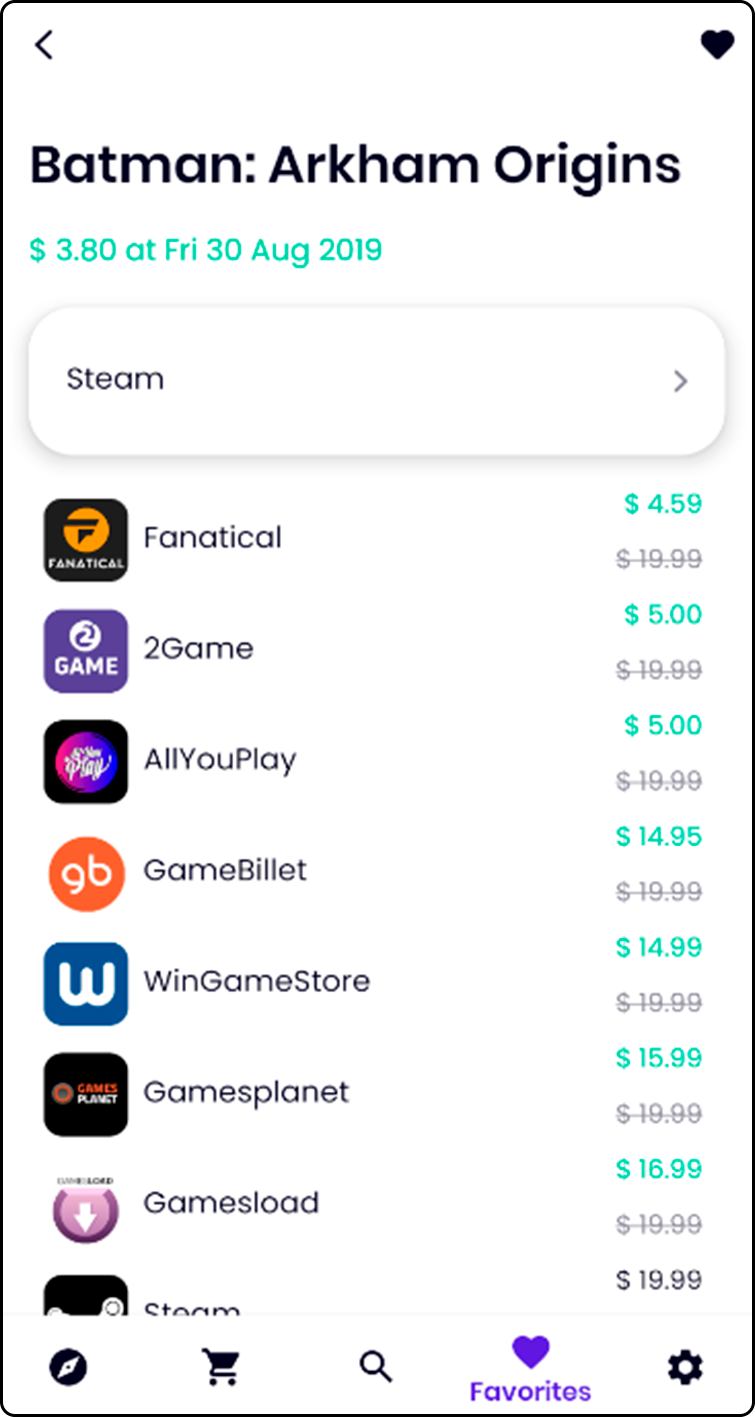
\includegraphics[scale=0.25]{favorites_3.png} 
   \caption{Информация об игре}
   \label{fig:arch:favorites_3}
\end{figure}

Если пользователь нажмёт на сохраненное предложение, то откроется экран с деталями об этом предложении. Пример пользовательского интерфейса представлен на рисунке~\ref{fig:arch:favorites_4}. На экране предложения присутствует лучшая цена за все времена, цена игры в магазине к которому предложение соответствует, а также индикация того, является ли это предложение лучшим среди магазинов. Если предложение является лучшим, то соответствующие сообщение показывается пользователю, если нет, то показывается список магазинов в котором эту игру можно купить по более дешевой цене.

\begin{figure}[H]
 \centering
   
\includegraphics[scale=0.25]{favorites_4.png} 
   \caption{Информация о предложении}
   \label{fig:arch:favorites_4}
\end{figure}


\undersection{Модуль поиска}~\par
Пользовательский интерфейс и программная реализация схожа с модулем избранного, за исключением наличия фильтров и возможности поиска. Приложение делает запросы на списки игр и предлжений вместе с фильтрами и поисковой строкой задаваемой пользователем. Стоит отметить, что поисковая строка реализована с соблюдением Google Material Design и содержит историю поисковых запросов пользователя, а также имеет возможность голосового ввода. Пример пользовательского интерфейса истории поисковых запросов представлен на рисунке~\ref{fig:arch:search_1}.

\begin{figure}[H]
 \centering
   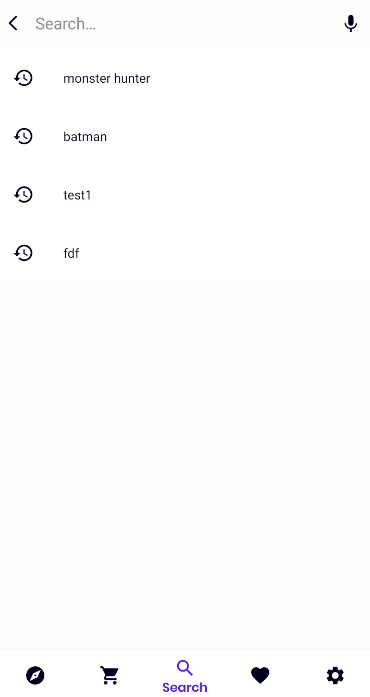
\includegraphics[scale=0.25]{search_1.png} 
   \caption{История поисковых запросов}
   \label{fig:arch:search_1}
\end{figure}

\undersection{Модуль магазинов}~\par
Модуль магазинов реализует получения списка всех доступных магазинов и возможность включать и отключать их при работе с приложением. Если пользователь выключит с помощью нажатия на кнопку какой-либо магазин, то он больше не будет участвовать в ответах выдываемых пользователю. Магазины могут работать в режиме без подключения к сети, для этого при получении магазинов производится их кеширование в локальную базу данных. При нажатии на один из магазинов открывается страница с предложениями только этого магазина. Пример пользовательского интерфейса представлен на рисунке~\ref{fig:arch:stores_2}.

\begin{figure}[H]
 \centering
   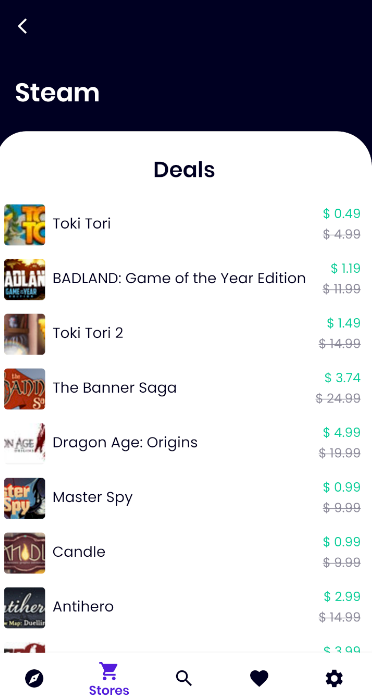
\includegraphics[scale=0.25]{stores_2.png} 
   \caption{Предложения одного магазина}
   \label{fig:arch:stores_2}
\end{figure}

\undersection{Модуль аккаунта}~\par
Модуль относящийся к настройкам самого пользователя и социальным функциям. Данный модуль аккаунта состоит из 6 экранов:

\begin{itemize}
    \item основной экран пользователя;
    \item экран нотификаций;
    \item экран с возможностью поделиться приложением;
    \item экран с возможностью купить подписку на приложение;
    \item экран настроек;
    \item экран информации.
\end{itemize}

Основной экран пользователя выполняет роль навигации между остальными экранами и позволяет сменить аватар пользователя. Пример пользовательского интерфейса представлен на рисунке~\ref{fig:arch:account_1}.

\begin{figure}[H]
 \centering
   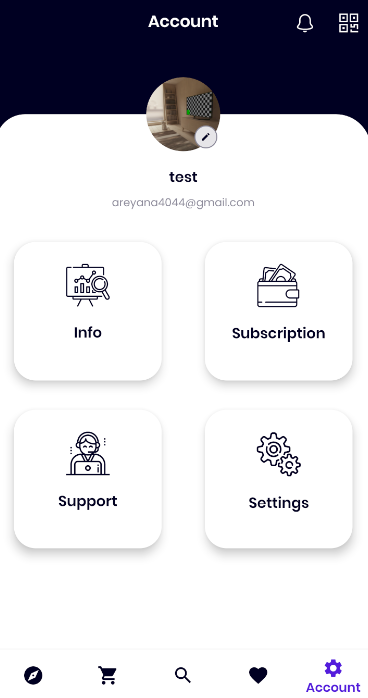
\includegraphics[scale=0.25]{account_1.png} 
   \caption{Основной экран пользователя}
   \label{fig:arch:account_1}
\end{figure}


Для данного экрана был написан набор методов по работе с камерой и галереей приложения. Пользователю доступны возможности удаления аватара, добавления его с помощью камеры или галереи приложения. Учтено отсутствия разрешний на камеру у приложения и выполнена обработка этой ситуации с помощью запрашивания этого разрешения у пользователя в виде диалога. Если пользователь отклонил 2 раза запрос разрешения на доступ к камере, то в следующие разы он будет получать сообщение о просьбе перехода на экран настроек приложения в системе Android и ручного добавления разрешения, данное действие происходит с помощью метода openSettingsPermissionAppActivity (см. листинг~\ref{lst:add:a_11}).

Одна из социальных функций приложения представлена в виде экрана с возможностью поделиться ссылкой на приложение в сообщении, либо QR кодом. Пример пользовательского интерфейса представлен на рисунке~\ref{fig:arch:account_5}.

\begin{figure}[H]
 \centering
   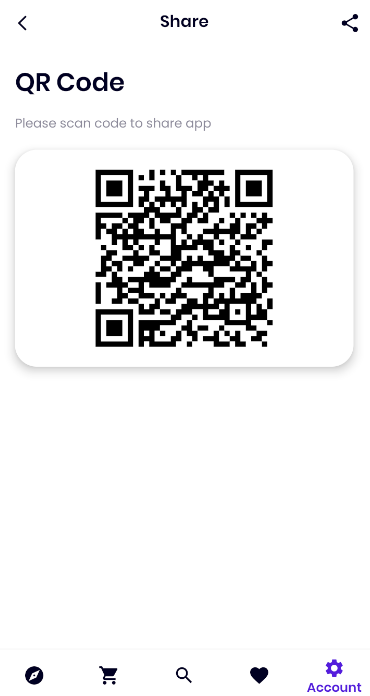
\includegraphics[scale=0.25]{account_5.png} 
   \caption{Экран с возможностью поделиться приложением}
   \label{fig:arch:account_5}
\end{figure}

С помощью нативного класса ShareCompat, был реализован метод по отправке ссылки на приложение. Ссылка может быть отправлена в любое приложение которое поддерживает тип test/plain (см. листинг~\ref{lst:share_method}).
\begin{lstlisting}[language=Java,label={lst:share_method},caption={Методы для отправки ссылки на приложение}]
            val shareItem = menu.findItem(R.id.menuShare)
            shareItem.setOnMenuItemClickListener {
                ShareCompat.IntentBuilder(requireContext())
                    .setType("text/plain")
                    .setChooserTitle("Choose one")
                    .setText("http://play.google.com/store/apps/details?id=" + requireActivity().packageName)
                    .startChooser()
                return@setOnMenuItemClickListener true
            }
\end{lstlisting}

В работе одним из самых важных экранов является экран настроек. Пример пользовательского интерфейса представлен на рисунке~\ref{fig:arch:account_2}. На экране присутствует список переходов и переключателей, данный список реализован с помощью библиотеки Groupie. Библиотека нужна для более удобного добавления новых опций в список без изменения большого количества кода.

\begin{itemize}
    \item переключатель Notification, включает и отключает доступ к нотификациям у приложения;
    \item переключатель Show inactive stores, изменяет видимость недоступных в данный момент магазинов в приложении;
    \item переход Language, осуществляет навигацию на экран смены языка приложения;
    \item переключатель Night mode, переключает с темной на светлую тему приложения и обратно;
    \item переход Privacy policy, осуществляет навигацию на страницу с политикой конфиденциальности;
    \item переход Terms of service, осущестлвяет навигацию на страницу с условиями обслуживания;
    \item переход Sign Out выполняет выход пользователя из приложения на модуль авторизации.
\end{itemize}

\begin{figure}[H]
 \centering
   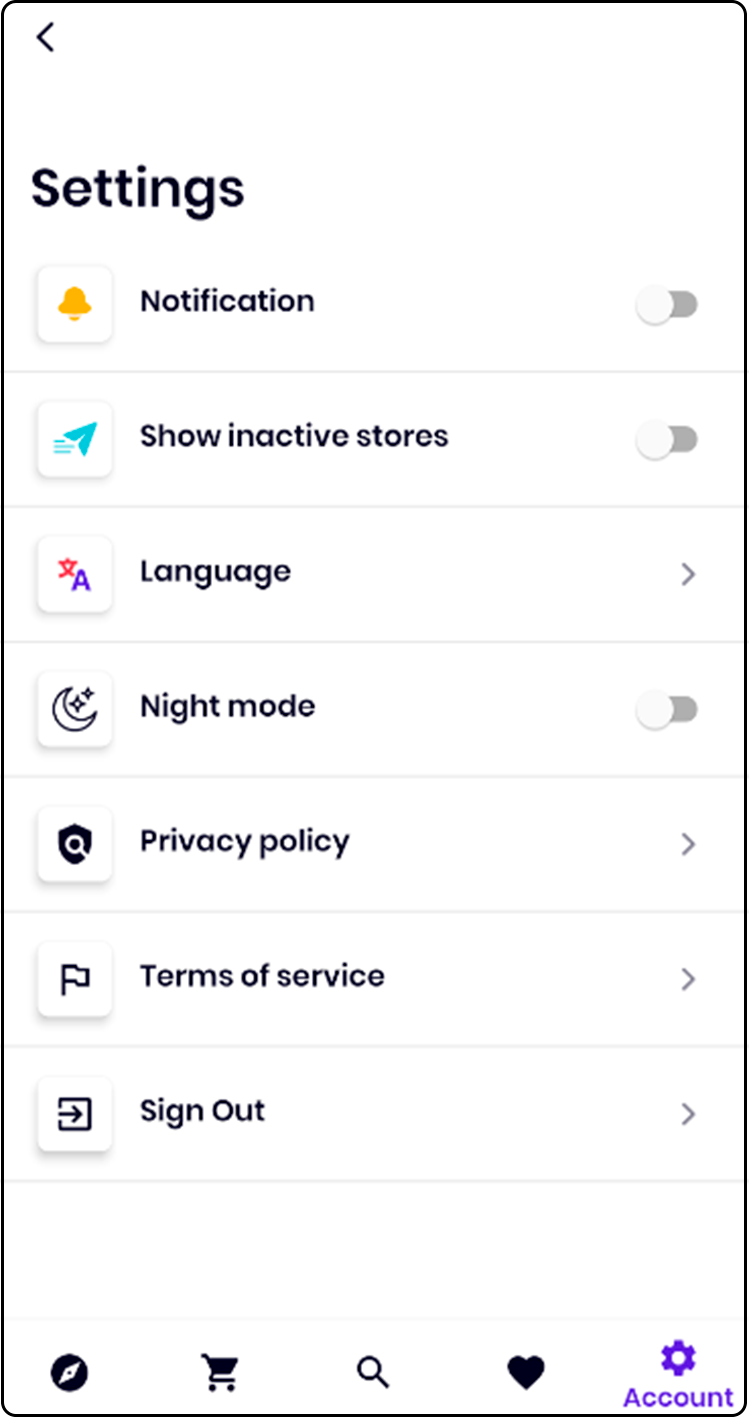
\includegraphics[scale=0.25]{account_2.png} 
   \caption{Экран настроек}
   \label{fig:arch:account_2}
\end{figure}

Каждая из настроек синхронизируется с Firestore для каждого пользователя, что позволяет сохранять состояние настроек на разных устройствах под одним аккаунтом. Например, для настройки Notification используется ключ notification под которым для каждого отдельного пользователя записывается состояние этой настройки с помощью методов putNotification и getNotification  (см. листинг~\ref{lst:prefs_notification}).

\begin{lstlisting}[language=Java,label={lst:prefs_notification},caption={Методы для Notification}]
    override suspend fun putNotification(boolean: Boolean) {
        return suspendCoroutine { cont ->
            val uid = auth.currentUser?.uid!!
            val users = db.collection(usersKey).document(uid)
            val map: Map<String, Boolean> = mapOf(notificationsKey to boolean)
            users.set(map, SetOptions.merge()).addOnCompleteListener {
                cont.resume(Unit)
            }.addOnCanceledListener {
                cont.resumeWithException(Exception("No Connection"))
            }
        }
    }

    override suspend fun getNotification(): Boolean {
        return suspendCoroutine { cont ->
            val uid = auth.currentUser?.uid!!
            val users = db.collection(usersKey).document(uid)
            users.get().addOnCompleteListener {
                if (it.isSuccessful && it.result != null) {
                    val result = it.result!!
                    if (result.contains(notificationsKey)) {
                        cont.resume(result[notificationsKey] as Boolean)
                    } else {
                        cont.resume(false)
                    }
                } else {
                    cont.resumeWithException(Exception("No Connection"))
                }
            }.addOnCanceledListener {
                cont.resumeWithException(Exception("No Connection"))
            }
        }
    }
\end{lstlisting}

На экране информации пользователь может прочитать о приложении и перейти по ссылкам чтобы получить связанную с разработчиком информацию, например на сервер Discord или в PlayStore. Переход по ссылкам осуществляется с помощью browserIntent, намерения с помощью которого система открывает ссылку в доступном браузере с использованием ACTION VIEW типа намерения (см. листинг~\ref{lst:prefs_intent}).

\begin{lstlisting}[language=Java,label={lst:prefs_intent},caption={browserIntent}]
        val browserIntent = Intent(Intent.ACTION_VIEW, Uri.parse("http://play.google.com/store/apps/dev?id=areyanainc"))
        startActivity(browserIntent)
\end{lstlisting}

\subsection{Безопасность}
Для обеспечения безопасности чувствительных данных была использована Android библиотека Security для шифрования пользовательских настроек приложения. Логика по взаимодействию с этой библиотекой реализована в классе PreferenceDataSource (см. листинг~\ref{lst:add:a_9}).

На серверной стороне для Firebase Storage и Firestore были написаны правила, которые не позволяют пользователям получать доступ ко всем данным, а только для их части, что соответствует их уникальному идентификатору (см. листинг~\ref{lst:firebase_security}).

\begin{lstlisting}[language=Javascript,label={lst:firebase_security},caption={Правила Firestore}]
rules_version = '2';
service cloud.firestore {
  match /databases/{database}/documents {
     match /users/{userId}/{document=**} {
      allow read, update, delete, create: if request.auth.uid == userId;
    }
  }
}
\end{lstlisting}


\subsection{Варианты использования}
Далее будут рассмотрены основные варианты использования разработанного мобильного приложения.

\undersection{ВИ Создание учётной записи}~\par
\label{use:reg}
Описание ВИ: Пользователь имеет возможность при желании создать личную учётную запись.
 
Предусловия основного потока действий нет.
 
Основной поток действий:
\begin{itemize}
   \item пользователь нажимает кнопку «Register»;
   \item пользователь вводит электронную почту, имя пользователя, пароль.
\end{itemize}
 
Ограничения: различные ограничения, установленные провайдером аутентификации Firebase, а также клиентским приложением.
 
\undersection{ВИ Использование своей учётной записи}~\par
Описание ВИ: Пользователь имеет возможность использовать личную учётную запись.
 
Предусловия основного потока действий: у пользователя имеется учётная запись.
 
Основной поток действий:
\begin{itemize}
   \item пользователь нажимает кнопку «SIGN IN»;
   \item пользователь вводит электронную почту и пароль.
\end{itemize}
 
Ограничения: различные ограничения, установленные провайдером аутентификации Firebase, а также клиентским приложением.

\undersection{ВИ Восстановление пароля}~\par
\label{use:resetpassword}
Описание ВИ: Пользователь имеет возможность восстановить пароль для своей учетной записи.
 
Предусловия основного потока действий: пользователь должен быть зарегистрирован.
 
Основной поток действий:
\begin{itemize}
   \item пользователь нажимает кнопку «Forgot password?»;
   \item пользователь вводит email своей учетной записи;
   \item клиент получает письмо на email с восстановлением пароля.
\end{itemize}
 
Ограничения: email должен быть валидным и не пустым.
 
\undersection{ВИ Просмотр истории}~\par
Описание ВИ: Пользователь имеет возможность просмотреть историю о вышедшей новинке.
 
Предусловия основного потока действий: у пользователя имеется учётная запись.
 
Основной поток действий:
\begin{itemize}
   \item пользователь нажимает на историю;
   \item пользователь получает на экран изображения игры в виде историй из Instagram;
   \item пользователь может совершать навигацию между изображениями с помощью жестов.
\end{itemize}
 
Ограничений нет.

\undersection{ВИ Просмотр статьи}~\par
\label{use:join}
Описание ВИ: Пользователь имеет возможность просмотреть свежую статью об игровой индустрии.
 
Предусловия основного потока действий: у пользователя имеется учётная запись.
 
Основной поток действий:
\begin{itemize}
   \item пользователь нажимает на статью;
   \item приложение открывает браузер со статьей.
\end{itemize}
 
Ограничения: пользователь должен иметь подключение к интернету.
 
\undersection{ВИ Просмотр предложения}~\par
Описание ВИ: Пользователь имеет возможность просмотреть дополнительную информацию о предложении.
 
Предусловия основного потока действий: у пользователя имеется учётная запись.

Основной поток действий:
\begin{itemize}
   \item пользователь нажимает на предложение;
   \item приложение совершает навигацию на страницу о дополнительной информации о предложении;
   \item приложение делает запрос о дополнительной информации о предложении;
   \item пользователь может просматривать дополнительную информацию о предложении, в виде скидок, более выгодных предложений, рейтинга.
\end{itemize}
 
Ограничения: пользователь должен иметь подключение к интернету.
 
\undersection{ВИ Просмотр игры}~\par
Описание ВИ: Пользователь имеет возможность просмотреть дополнительную информацию об игре.
 
Предусловия основного потока действий: у пользователя имеется учётная запись.

Основной поток действий:
\begin{itemize}
   \item пользователь нажимает на игру;
   \item приложение совершает навигацию на страницу о дополнительной информации о игре;
   \item приложение делает запрос о дополнительной информации об игре;
   \item пользователь может просматривать дополнительную информацию об игре, в виде скидок, предложений, рейтинга.
\end{itemize}
 
Ограничения: пользователь должен иметь подключение к интернету.
 
\undersection{ВИ Просмотр списка магазинов}~\par
\label{use:showstores}
Описание ВИ: Пользователь имеет возможность просмотреть все магазины доступные в приложении.
 
Предусловия основного потока действий: у пользователя имеется учётная запись.
 
Основной поток действий:
\begin{itemize}
   \item пользователь открывает список магазинов;
   \item приложение делает запрос на список магазинов;
   \item приложение отображает список магазинов;
   \item пользователь может просматривать список магазинов.
\end{itemize}
 
Ограничения: пользователь должен иметь подключение к интернету.

\undersection{ВИ Просмотр отдельного магазина}~\par
\label{use:singlestore}
Описание ВИ: Пользователь имеет возможность просмотреть предложения конкретного магазина.
 
Предусловия основного потока действий: у пользователя имеется учётная запись, пользователь просматривает список магазинов.
 
Основной поток действий:
\begin{itemize}
   \item пользователь нажимает на отдельный магазин;
   \item приложение делает запрос на список предложений от конкретного магазина;
   \item приложение показывает список предложений от конкретного магазина;
   \item пользователь может просматривать и выбирать предложения.
\end{itemize}
 
Ограничения: пользователь должен иметь подключение к интернету.

\undersection{ВИ Выключение магазина из фильтрации}~\par
Описание ВИ: Пользователь имеет возможность выключить магазин из фильтрации в приложении.
 
Предусловия основного потока действий: у пользователя имеется учётная запись, Пользователь просматривает список магазинов.
 
Основной поток действий:
\begin{itemize}
   \item пользователь нажимает на checkbox, тем самым выключая магазин из фильтрации;
   \item приложение запоминает выбор пользователя.
\end{itemize}

Альтернативный поток действий:
\begin{itemize}
   \item пользователь нажимает на checkbox, тем самым включая магазин в фильтрацию;
   \item приложение запоминает выбор пользователя.
\end{itemize}
 
Ограничений нет.

\undersection{ВИ Поиск игр}~\par
\label{use:searchgames}
Описание ВИ: Пользователь имеет возможность совершать поиск по играм с помощью поисковой строки и фильтров.
 
Предусловия основного потока действий: у пользователя имеется учётная запись.
 
Основной поток действий:
\begin{itemize}
   \item пользователь открывает поиск;
   \item приложение делает запрос на список игр;
   \item пользователь вводит в поисковую строку значения и выбирает фильтр;
   \item приложение показывает список отфильтрованных игр;
   \item пользователь может просматривать список отфильтрованных игр.
\end{itemize}
 
Ограничения: пользователь должен иметь подключение к интернету.

\undersection{ВИ Поиск предложений}~\par
\label{use:searchdeals}
Описание ВИ: Пользователь имеет возможность совершать поиск по предложениям с помощью поисковой строки и фильтров.
 
Предусловия основного потока действий: у пользователя имеется учётная запись.
 
Основной поток действий:
\begin{itemize}
   \item пользователь открывает поиск;
   \item приложение делает запрос на список предложений;
   \item пользователь вводит в поисковую строку значения и выбирает фильтр;
   \item пользователь может просматривать список отфильтрованных предложений.
\end{itemize}
 
Ограничения: пользователь должен иметь подключение к интернету.

\undersection{ВИ Добавление предложения в избранное}~\par
\label{use:favoritedeals}
Описание ВИ: Пользователь имеет возможность добавить в избранное предложение.
 
Предусловия основного потока действий: у пользователя имеется учётная запись, пользователь совершил поиск по предложениям.
 
Основной поток действий:
\begin{itemize}
   \item пользователь нажимает на предложение из списка;
   \item пользователь нажимает на кнопку избранного и добавляет предложение в избранное;
   \item приложение запоминает выбор пользователя.
\end{itemize}

Альтернативный поток действий:
\begin{itemize}
   \item пользователь нажимает на предложение из списка;
   \item пользователь нажимает на кнопку избранного и удаляет предложение из избранного;
   \item приложение запоминает выбор пользователя.
\end{itemize}

Ограничения: пользователь должен иметь подключение к интернету.

\undersection{ВИ Добавление игры в избранное}~\par
\label{use:favoritegames}
Описание ВИ: Пользователь имеет возможность добавить в избранное игру.
 
Предусловия основного потока действий: у пользователя имеется учётная запись, пользователь совершил поиск по играм.
 
Основной поток действий:
\begin{itemize}
   \item пользователь нажимает на игру из списка;
   \item пользователь нажимает на кнопку избранного и добавляет игру в избранное;
   \item приложение запоминает выбор пользователя.
\end{itemize}

Альтернативный поток действий:
\begin{itemize}
   \item пользователь нажимает на игру из списка;
   \item пользователь нажимает на кнопку избранного и удаляет игру из избранного;
   \item приложение запоминает выбор пользователя.
\end{itemize}

Ограничения: пользователь должен иметь подключение к интернету.

\subsection{Тестирование приложения}
Для оптимизации мобильного приложения использовалось программное обеспечение из проекта Leak Canary. В рамках данного проекта разработан набор различных программ, которые помогают автоматизировать процесс тестирования мобильных приложений. Для данного проекта использовались JUnit и Espresso которые являются универсальными библиотеками для тестирования мобильных приложений.

JUnit~-- библиотека позволяющая проводить модульное тестирование отдельных частей приложения. С помощью данной библиотеки проводится тестирование отдельных объектов выбранного класса и его методов. Модульное тестирование позволяет покрыть до в среднем до 90\% бизнес-логики любого программного обеспечения, за исключением сложных UI тестов.

Espresso~-- фреймворк для тестирования UI/UX приложения. Данный фреймворк устраняет недочеты JUnit в виде тестирование интерфейсов и предоставляет удобный интерфейс для написания тестов. Пользователю фреймворка нет надобности в проверках фокусов и доступности отдельных кнопок и других элементов интерфейса, фреймворк делает это за пользователя. В совокупности с JUnit, Espresso предоставляет возможность покрыть тестами всё приложение и упростить будущее расширение модулей приложения и их тестирование.
 
Также было проведено ручное тестирование приложения, так как при помощи тестов Android некоторые моменты протестировать затруднительно. В рамках ручного тестирования было проведено дымовое тестирование возможностей приложения и механизмов синхронизации.


%Примеры пользовательского интерфейса представлены на рисунках~\ref{fig:arch:main_page} и~\ref{fig:arch:room_page}.
%Для воспроизведения видео используется тег <video>, который был введён в стандарте HTML5.
%
%Данный стандарт определяет для тега <video> ряд атрибутов и событий, для контроля воспроизведения.
%Проблема заключается в том, что стандартные элементы управления тега <video> не обладают всеми необходимыми возможностями для реализации данного проекта.
%Также при помощи JS кода нет никакой возможности изменить события при взаимодействии со стандартные элементы управления. 
%Можно только добавить собственную логику, которая будет работать после выполнения стандартной.
%Данное ограничение делает невозможным реализацию хорошей синхронизации, так как у пользователя инициировавшего событие оно произойдёт сразу, а у остальных после %получения данных с сервера.
%
%Для решения проблемы синхронизации был реализован собственный пользовательский интерфейс (см. рис.~\ref{fig:arch:room_page}), который позволяет полностью манипулировать %порядком выполняемых действий. Реализация данного пользовательского интерфейса представлена в листинге~\ref{lst:player}.
%\begin{lstlisting}[language=JavaScript,label={lst:player},caption={Компонент Player}]
%    import React, { Component } from 'react';
%    import { MdPlayArrow, MdPause, MdFullscreen, MdQueue } from 'react-icons/md';
%    import './player.scss';
%    import TimeIndicator from './TimeIndicator';
%    import RangeBar from './Slider';
%    import Hotkeys from 'react-hot-keys';
%    import VolumeSlider from './VolumeSlider';
%    import { PlayerBackend } from '../PlayerBackend/default';
%    import PlayList from './PlayList';
%    import Notifications from './Notifications';
%    import Chat from './Chat';
%     
%    const pauseIcon = <MdPause />;
%    const playIcon = <MdPlayArrow />;
%     
%    class Player extends Component {
%       constructor(props) {
%           super(props);
%           this.processor = new PlayerBackend();
%           this.playerElemetn = React.createRef();
%           this.state = {
%               isFullscreen: false,
%               playbackIcon: playIcon,
%               playbackState: false,
%               playlist: false,
%               showVideoChooser: false,
%               showChat: false,
%           }
%       }
%     
%       componentDidMount() {
%           this.vid_title = document.getElementById('video-title');
%           this._connectToPlayerBackend();
%           document.onfullscreenchange = () => this.setState({ isFullscreen: !this.state.isFullscreen });
%           if (this.props.externalSetUp) {
%               for (const func of this.props.externalSetUp) {
%                   func(this.processor);
%               }
%           }
%       }
%     
%       _connectToPlayerBackend = () => {
%           this.processor.video = document.getElementById('video-player');
%           this.setState({ time: this.processor.time, volume: this.processor.volume })
%     
%           this.processor.video.addEventListener('timeupdate', () => this.setState({ time: this.processor.time }));
%           this.processor.video.addEventListener('volumechange', () => this.setState({ volume: this.processor.volume }));
%     
%           for (const event in this.props.events) {
%               this.processor.addPreAction(this.props.events[event], event);
%           }
%       }
%     
%       playback = () => {
%           this.processor.dispatch('changePlayback', this.processor.paused);
%           this.processor.dispatch('setTime', this.processor.time);
%           let newIcon = this.processor.paused ? pauseIcon : playIcon;
%           this.setState({ playbackIcon: newIcon, playbackState: this.processor.paused });
%       }
%     
%       fullscreen = () => {
%           if (this.state.isFullscreen) {
%               this.leaveFullscreen();
%           } else {
%               this.enterFullscreen();
%           }
%       }
%     
%       enterFullscreen = () => {
%           const elem = this.playerElemetn.current;
%           if (elem.requestFullscreen) {
%               elem.requestFullscreen();
%           } else if (elem.mozRequestFullScreen) {
%               elem.mozRequestFullScreen();
%           } else if (elem.webkitRequestFullscreen) {
%               elem.webkitRequestFullscreen();
%           } else if (elem.msRequestFullscreen) {
%               elem.msRequestFullscreen();
%           }
%       }
%     
%       leaveFullscreen = () => {
%           if (document.exitFullscreen) {
%               document.exitFullscreen();
%           } else if (document.mozCancelFullScreen) {
%               document.mozCancelFullScreen();
%           } else if (document.webkitExitFullscreen) {
%               document.webkitExitFullscreen();
%           } else if (document.msExitFullscreen) {
%               document.msExitFullscreen();
%           }
%       }
%     
%       setTime = (timeValue) => {
%           if (!timeValue.isNaN) {
%               this.processor.dispatch('setTime', timeValue * this.processor.duration);
%           }
%       }
%     
%       setVolume = (volumeValue) => {
%           this.processor.dispatch('setVolume', volumeValue);
%       }
%     
%       changeMute = () => {
%           this.processor.dispatch('changeMute');
%       }
%     
%     
%       togglePlaylist = () => {
%           this.setState({ playlist: !this.state.playlist });
%       }
%     
%       toogleChat = (e) => {
%           this.setState({ showChat: !this.state.showChat });
%       }
%     
%       render() {
%           return (
%               <div className='player-wrapper' id='player' ref={this.playerElemetn}>
%                   <Hotkeys keyName='space' onKeyUp={this.playback} />
%                   <Hotkeys keyName='c' onKeyUp={this.toogleChat} />
%                   <div className='player-layer'>
%                       <video id='video-player' />
%                   </div>
%     
%                   <div className='player-layer mouse-show'>
%                       <div id='player-controls' className='player-controls'>
%                           <div className='player-controls-row'>
%                               <RangeBar value={this.processor.timeProgress} handle_change={this.setTime} style={{ 'margin-top': '5px', 'margin-bottom': '5px' }} />
%                           </div>
%                           <div className='player-controls-row'>
%                               <div onClick={this.playback} className="player-button player-button-play">
%                                   {this.state.playbackIcon}
%                               </div>
%                               <VolumeSlider volume={this.state.volume} volumeHandler={this.setVolume} toggleMute={this.changeMute} />
%                               <TimeIndicator time={this.processor.time} duration={this.processor.duration} />
%                               <div className='player-button' onClick={this.togglePlaylist}>
%                                   <MdQueue />
%                               </div>
%                               <div id='fullscreen-btn' onClick={this.fullscreen} className="player-button player-button-fullscreen">
%                                   <MdFullscreen />
%                               </div>
%                           </div>
%                       </div>
%                   </div>
%                   <Notifications />
%                   <PlayList processor={this.processor} visibility={this.state.playlist} playlistLogic={this.props.playlistLogic} libraryLogic={this.props.libraryLogic} %toogleVideoChooser={this.toogleVideoChooser} />
%                   {this.state.showChat &&
%                       <div className='player-layer'>
%                           <Chat hide={this.toogleChat}/>
%                       </div>
%                   }
%               </div>
%           );
%       }
%    }
%     
%    export default Player;
%\end{lstlisting}
%
%Данный компонент содержит внутри себя несколько дочерних компонентов: PlayList, VolumeSlider, TimeIndicator, RangeBar. 
%Это сделано с целью оптимизации работы с деревом DOM, так как данные элементы должны регулярно обновляться.
%
%Элементы управления компонента Player обрабатывают определённые события (пауза, перемотка и т.д.). 
%Для непосредственного управления тегом <video> реализован дополнительный класс PlayerBackend (см. листинг~\ref{lst:playerback}), который содержит логику для управления %процессом воспроизведения. При помощи данного класса можно управлять видео напрямую, вызывая событие сразу, или использовать метод dispatch, который занимается %обработкой последовательности событий.
%Данный метод необходим для того, чтобы можно было модифировать стандартную логику тега <video>.
%При реализации данного метода ыл рассмотрен механизм работы библиотеки Redux, для того чтобы данный метод соответствовал Flux архитектуре.
%Для метода dispatch доступно следующие действия (actions): 
%\begin{itemize}
%    \item changePlayback (ставит видео на паузу или возобновляет воспроизведение);
%    \item setTime (перематывает видео);
%    \item setVolume (изменяет громкость видео);
%    \item changeMute (заглушает видео);
%    \item setSrc (устанавливает источник видео).
%\end{itemize}
%
%Метод dispatch позволяет выполнить дополнительное действие перед стандартным. Для этого необходимо после создания объекта данного класса вызвать метод addPreAction, %который принимает название действия и функцию, которую необходимо выполнить перед данным действием. Благодаря этому разработанный плеер можно использовать и без %синхронизации, так как синхронизирующая логика добавляется при помощи метода addPreAction.
%
%\begin{lstlisting}[language=JavaScript,label={lst:playerback},caption={Класс PlayerBackend}]
%class PlayerBackend {
% constructor(video) {
%     this._video = video;
%     this._preActions = {};
%     this._actions = {
%         'changePlayback': this.changePlayback,
%         'setTime': this.setTime,
%         'setVolume': this.setVolume,
%         'changeMute': this.changeMute,
%         'setSrc': this.setSource
%     }
% }
% 
% set video(value) {
%     this._video = value;
%     this._video.addEventListener('error', (e) => { console.error('error', e) });
%     this._video.addEventListener('waiting', (e) => { console.error('waiting', e) });
%     this._video.addEventListener('stalled', (e) => { console.error('stalled', e) });
% }
% 
% get video() {
%     return this._video;
% }
% 
% addPreAction = (value, action) => {
%     if (this._preActions[action] === undefined) {
%         this._preActions[action] = []
%     }
%     this._preActions[action].push(value);
% }
% 
% resetPreActions() {
%     this._preActions = {}
% }
% 
% resetPostActions() {
%     this._preActions = {}
% }
% 
% // Playback
% _play = () => {
%     this._video.play().catch((e) => console.error('playback', e));
% }
% 
% _pause = () => {
%     this._video.pause();
% }
% 
% get paused() {
%     return this._video.paused;
% }
% 
% changePlayback = (paused) => {
%     if (paused !== undefined) {
%         paused ? this._play() : this._pause();
%     } else {
%         this.paused ?  this._play() : this._pause();
%     }
% }
% 
% // Volume
% set volume(value) {
%     this._video.volume = value;
% }
% 
% setVolume = (value) => this._video.volume = value;
% 
% get volume() {
%     return this._video.volume;
% }
% 
% get muted() {
%     return this._video.muted;
% }
% 
% changeMute = () => {
%     this._video.muted = !this._video.muted;
% }
% 
% // Time
% setTime = (value) => this._video.currentTime = value;
%  set time(value) {
%     this._video.currentTime = value;
% }
% 
% setTime = (value) => this._video.currentTime = value;
% 
% get time() {
%     return this._video ? this._video.currentTime || 0 : 0;
% }
% 
% get timeProgress() {
%     return this._video ? this._video.currentTime / this._video.duration || 0 : 0;
% }
% 
% get duration() {
%     return this._video ? this._video.duration || 0 : 0;
% }
% 
% //  Src
% set source(value) {
%     this._video.src = value;
% }
% 
% setSource = (value) => this._video.src = value;
% 
% dispatch = (action, value) => {
%     let _preActions = this._preActions[action] || [];
%     const _actionWrapper = promiseWrapper(this._actions[action], value);
% 
%     let promise = new Promise(resolve => resolve());
%     for (const _preAction of _preActions) {
%         promise = promise.then(promiseWrapper(_preAction, value));
%     }
% 
%     promise.then(promiseWrapper(this._actions[action], value));
% }
%}
%\end{lstlisting}
%
%\subsection{Реализация синхронизирующей логики}
%Так как класс PlayerBackend позволяет выполнять основные операции для управления видео без синхронизации, для выполнения синхронизации необходимо использовать %дополнительный класс, который предоставит данную возможность. Реализация основных методов для синхронизации и работы с Firebase представлена в листинге~\ref{lst:firebase}%. 
%
%\begin{lstlisting}[language=JavaScript,label={lst:firebase},caption={Методы для взаимодействия с Firebase}]
%changePlayback = (roomId, paused) => {
% let room_ref = this.db.collection('rooms').doc(roomId);
% room_ref.update({ paused })
% return room_ref.get().then(() => 'skip');
%}
% 
%listenPlayback = (roomId, dispatcher) => {
% return this.db.collection('rooms').doc(roomId).onSnapshot(snap => {
%   if (snap.data()) {
%     dispatcher.firebaseData.paused = snap.data().paused;
%     dispatcher.changePlayback(!snap.data().paused);
% 
%   }
% });
%}
% 
%getPlayback = (roomId, dispatcher) => {
% let roomRef = this.db.collection('rooms').doc(roomId);
% return roomRef.get().then(value => dispatcher.changePlayback(!value.data().paused));
%}
% 
%setTime = (roomId, time) => {
% let room_ref = this.db.collection('rooms').doc(roomId);
% room_ref.update({ time })
% return room_ref.get().then(() => 'skip');
%}
% 
%listenTime = (roomId, dispatcher) => {
% return this.db.collection('rooms').doc(roomId).onSnapshot(snap => {
%   if (snap.data()) {
%     if (dispatcher.firebaseData.time !== snap.data().time || dispatcher.firebaseData.src != snap.data().src) {
%       dispatcher.firebaseData.time = snap.data().time;
%       dispatcher.setTime(snap.data().time)
%     }
% 
%   }
% });
%}
% 
%getTime = (roomId, dispatcher) => {
% let roomRef = this.db.collection('rooms').doc(roomId);
% return roomRef.get().then(value => dispatcher.setTime(value.data().time || 0));
%}
% 
%listenSrc = (roomId, dispatcher) => {
% return this.db.collection('rooms').doc(roomId).onSnapshot(snap => {
%   if (snap.data()) {
%     if (dispatcher.firebaseData.src !== snap.data().src) {
%       dispatcher.firebaseData.src = snap.data().src;
%       dispatcher.setSource(snap.data().src)
%     }
%   }
% });
%}
% 
%setSrc = (roomId, src) => {
% let room_ref = this.db.collection('rooms').doc(roomId);
% let roomInfoRef = this.db.collection('roominfo').doc(roomId);
% room_ref.update({ src })
% roomInfoRef.update({ src });
% return room_ref.get().then(() => 'skip');
%}
% 
%listenPlaylist = (roomId, controller) => {
% let playlistRef = this.db.collection('playlists').doc(roomId);
% return playlistRef.onSnapshot(snap => {
%   if (snap.data()) {
%     controller(snap.data().videos)
%   }
% })
%}
% 
%addItemsToPlaylist = (playlistId, items) => {
% let playlistRef = this.db.collection('playlists').doc(playlistId);
% return playlistRef.update({ videos: firebase.firestore.FieldValue.arrayUnion(...items) });
%}
% 
%removeItemsFromPlaylist = (playlistId, items) => {
% let playlistRef = this.db.collection('playlists').doc(playlistId);
% playlistRef.update({
%   videos: firebase.firestore.FieldValue.arrayRemove(...items)
% })
%}
% 
%setPlaylist = (playlistId, playlist) => {
% let playlistRef = this.db.collection('playlists').doc(playlistId);
% return playlistRef.update({ videos: playlist });
%}
% 
%addUserToRoom = (roomId) => {
% let user = this.auth.currentUser;
% console.log('user', user)
% if (user) {
%   let statsRef = this.db.collection('stats').doc(roomId);
%   statsRef.update({
%     users: firebase.firestore.FieldValue.arrayUnion({ id: user.uid, status: null })
%   });
% }
%}
% 
%removeUserFromRoom = (roomId) => {
% let user = this.auth.currentUser;
% if (user) {
%   let statsRef = this.db.collection('stats').doc(roomId);
%   statsRef.update({
%     users: firebase.firestore.FieldValue.arrayRemove({ id: user.uid, status: null })
%   });
% }
%}
% 
%createRoom = (name, usePassword, password) => {
% if (!this.auth.currentUser.isAnonymous) {
%   return this.db.collection('roominfo').where('owner', '==', this.auth.currentUser.uid).get().then((querySnap) => {
%     if (querySnap.size < 1) {
%       return this.db.collection('roominfo').add({
%         name,
%         usePassword,
%         password,
%         users: [],
%         hidden: false,
%         src: '',
%         owner: this.auth.currentUser.uid,
%       }).then(docRef => {
%         this.db.collection('rooms').doc(docRef.id).set({ paused: true, src: '', time: 0, })
%         this.db.collection('messages').doc(docRef.id).set({ messages: [] });
%         this.db.collection('videos').doc(docRef.id).set({ videos: [] });
%       });
%     } else {
%       throw Error("You can't create more rooms")
%     }
%   })
% 
% }
%}
% 
%listenRooms = (controller) => {
% return this.db.collection('roominfo').onSnapshot(snap => {
%   let rooms = [];
%   snap.forEach(doc => {
%     rooms.push({ ...doc.data(), id: doc.id });
%   })
%   controller(rooms);
% });
%}
% 
%listenRoom = (roomId, controller) => {
% return this.db.collection('roominfo').doc(roomId).onSnapshot(snap => {
%   if (snap.data()) {
%     controller(snap.data());
%   }
% })
%}
% 
%getRoom = (roomId) => {
% return this.db.collection('roominfo').doc(roomId).get().then(doc => {
%   return doc.data();
% });
%}
% 
%getUserRooms = (userId) => {
% return this.db.collection('roominfo').where('owner', '==', userId || '').get().then((querySnap) => {
%   const rooms = []
%   querySnap.forEach(doc => {
%     rooms.push(doc.data());
%   })
%   return rooms;
% })
%}
% 
%enterRoom = (roomId, password) => {
% let docRef = this.db.collection('roominfo').doc(roomId)
% return docRef.get().then(doc => {
%   let result = true;
%   if (doc.data().usePassword && password !== doc.data().password) {
%     result = false;
%   }
%   return result;
% })
%}
% 
%findRoom = (query) => {
% return this.db.collection('roominfo').get().then(snap => {
%   let result = [];
% 
%   snap.forEach(docRef => {
%     if (docRef.data().name.includes(query)) {
%       result.push(docRef.data());
%     }
%   });
% 
%   return result;
% })
%}
% 
%listenChat = (roomId, controller) => {
% return this.db.collection('messages').doc(roomId).onSnapshot(snap => {
%   controller(snap.data().messages);
% });
%}
%\end{lstlisting}
%
%Для того, чтобы пользователь получал синхронизирующие данные от других пользователей используются методы: listenPlayback, listenTime и\linebreak listenSrc. 
%Данные методы инициализируют соединение с Firebase и при помощи методов из класса PlayeBackend изменяют состояние воспроизведения видео в зависимости от текущих данных %на сервере. 
%Данные методы гарантируют, что все пользователи комнаты будут получать информацию о состоянии воспроизведения с сервера. 
%Данные методы вызываются при подключении пользователя к комнате. 
%Для отправки запроса об изменении состояния воспроизведения используются методы: changePlayback, setTime и setSrc. 
%Данные методы берут значение текущего состояния видео и оправляют эти значения в Firebase. 
%При помощи идентификатора комнаты данные значения записываются в необходимый документ коллекции rooms. 
%Данные из этих документов затем получают методы listenPlayback, listenTime и listenSrc. Которые затем вызывают необходимые действия класса PlayerBackend. 
%Для вызова методов changePlayback, setTime и setSrc из модуля Firebase используется метод dispatch класса PlayerBackend. 
%Это позволяет выполнять синхронизирующие вызовы только когда пользователь находиться в комнате.
%
%Для того чтобы установить синхронизирующую логику для компонента Player используется компонент обёртка FirebasePlayer (см. листинг~\ref{lst:fplayer}). 
%Данный компонент устанавливает идентификатор комнаты для методов Firebase и затем передаёт их компоненту Player, где те устанавливаются как обработчики действий в классе %PlayerBackend.
%\begin{lstlisting}[language=JavaScript,label={lst:fplayer},caption={Компонент FirebasePlayer}]
%    class FirebasePlayer extends PureComponent {
%        constructor(props) {
%            super(props);
%            if (props.roomId) {
%                this.events = {
%                    'changePlayback': this.firebasePlayback,
%                    'setTime': this.firebaseTime,
%                    'setSrc': this.firebaseSource,
%                }
%                this.setUp = [this.setUpFirebaseData, this.firebaseListenSource, this.firebaseListenPlayback, this.firebaseListenTime]
%                this.libraryLogic = {
%                    'getLibraryItem': this.firebaseGetLibraryItem
%                }
%                this.playlistLogic = {
%                    'listenPlaylist': this.firebaseListenPlaylist,
%                    'addItems': this.firebaseAddItemsToPlaylist,
%                    'removeItems': this.firebaseRemoveItemsFromPlaylist,
%                    'setPlaylist': this.firebaseSetPlaylist,
%                }
%            }
%        }
%    
%        componentDidMount() {
%            if (this.props.roomId) {
%                this.props.firebase.sign_in_anon().then(() => {
%                    this.props.firebase.addUserToRoom(this.props.roomId);
%                })
%                window.addEventListener('beforeunload', () => this.props.firebase.removeUserFromRoom(this.props.roomId));
%    
%            }
%        }
%    
%        componentWillMount() {
%            if (this.props.roomId) {
%                window.removeEventListener('beforeunload', () => this.props.firebase.removeUserFromRoom(this.props.roomId));
%                this.props.firebase.removeUserFromRoom(this.props.roomId);
%    
%            }
%        }
%    
%        firebaseSetPlaylist = (playlist) => {
%            return this.props.firebase.setPlaylist(this.props.roomId, playlist);
%        }
%    
%        firebaseRemoveItemsFromPlaylist = (items) => {
%            return this.props.firebase.removeItemsFromPlaylist(this.props.roomId, items);
%        }
%    
%        firebasePlayback = (value) => {
%            return this.props.firebase.changePlayback(this.props.roomId, !value)
%        }
%    
%        firebaseListenPlayback = (dispatcher) => {
%            return this.props.firebase.listenPlayback(this.props.roomId, dispatcher);
%        }
%    
%        fetchPlayback = (dispatcher) => {
%            return this.props.firebase.getPlayback(this.props.roomId, dispatcher);
%        }
%    
%        firebaseTime = (value) => {
%            return this.props.firebase.setTime(this.props.roomId, value)
%        }
%    
%        firebaseListenTime = (dispatcher) => {
%            return this.props.firebase.listenTime(this.props.roomId, dispatcher);
%        }
%    
%        setUpFirebaseData = (dispatcher) => {
%            dispatcher.firebaseData = {}
%        }
%    
%        firebaseSource = (value) => {
%            return this.props.firebase.setSrc(this.props.roomId, value);
%        }
%    
%        firebaseListenSource = (dispatcher) => {
%            return this.props.firebase.listenSrc(this.props.roomId, dispatcher);
%        }
%    
%        firebaseGetLibraryItem = (id) => {
%            return this.props.firebase.getLibraryItem(id).then(value => value)
%        }
%    
%        firebaseListenPlaylist = (controller) => {
%            return this.props.firebase.listenPlaylist(this.props.roomId, controller)
%        }
%    
%        firebaseAddItemsToPlaylist = (items) => {
%            return this.props.firebase.addItemsToPlaylist(this.props.roomId, items)
%        }
%    
%        render() {
%            return (
%                <div className='f-player'>
%                    <Player events={this.events} externalSetUp={this.setUp} libraryLogic={this.libraryLogic} playlistLogic={this.playlistLogic} />
%                </div>
%            )
%        }
%    }
%\end{lstlisting}
%    
%
%\subsection{Клиентское веб-приложение}
%Клиентское приложение можно разделить на две структурные единицы: основная страница и страница комнаты. Примеры пользовательского интерфейса данных страниц представлены %на рисунках~\ref{fig:arch:main_page} и~\ref{fig:arch:room_page}
% 
%\begin{figure}[H]
% \centering
%   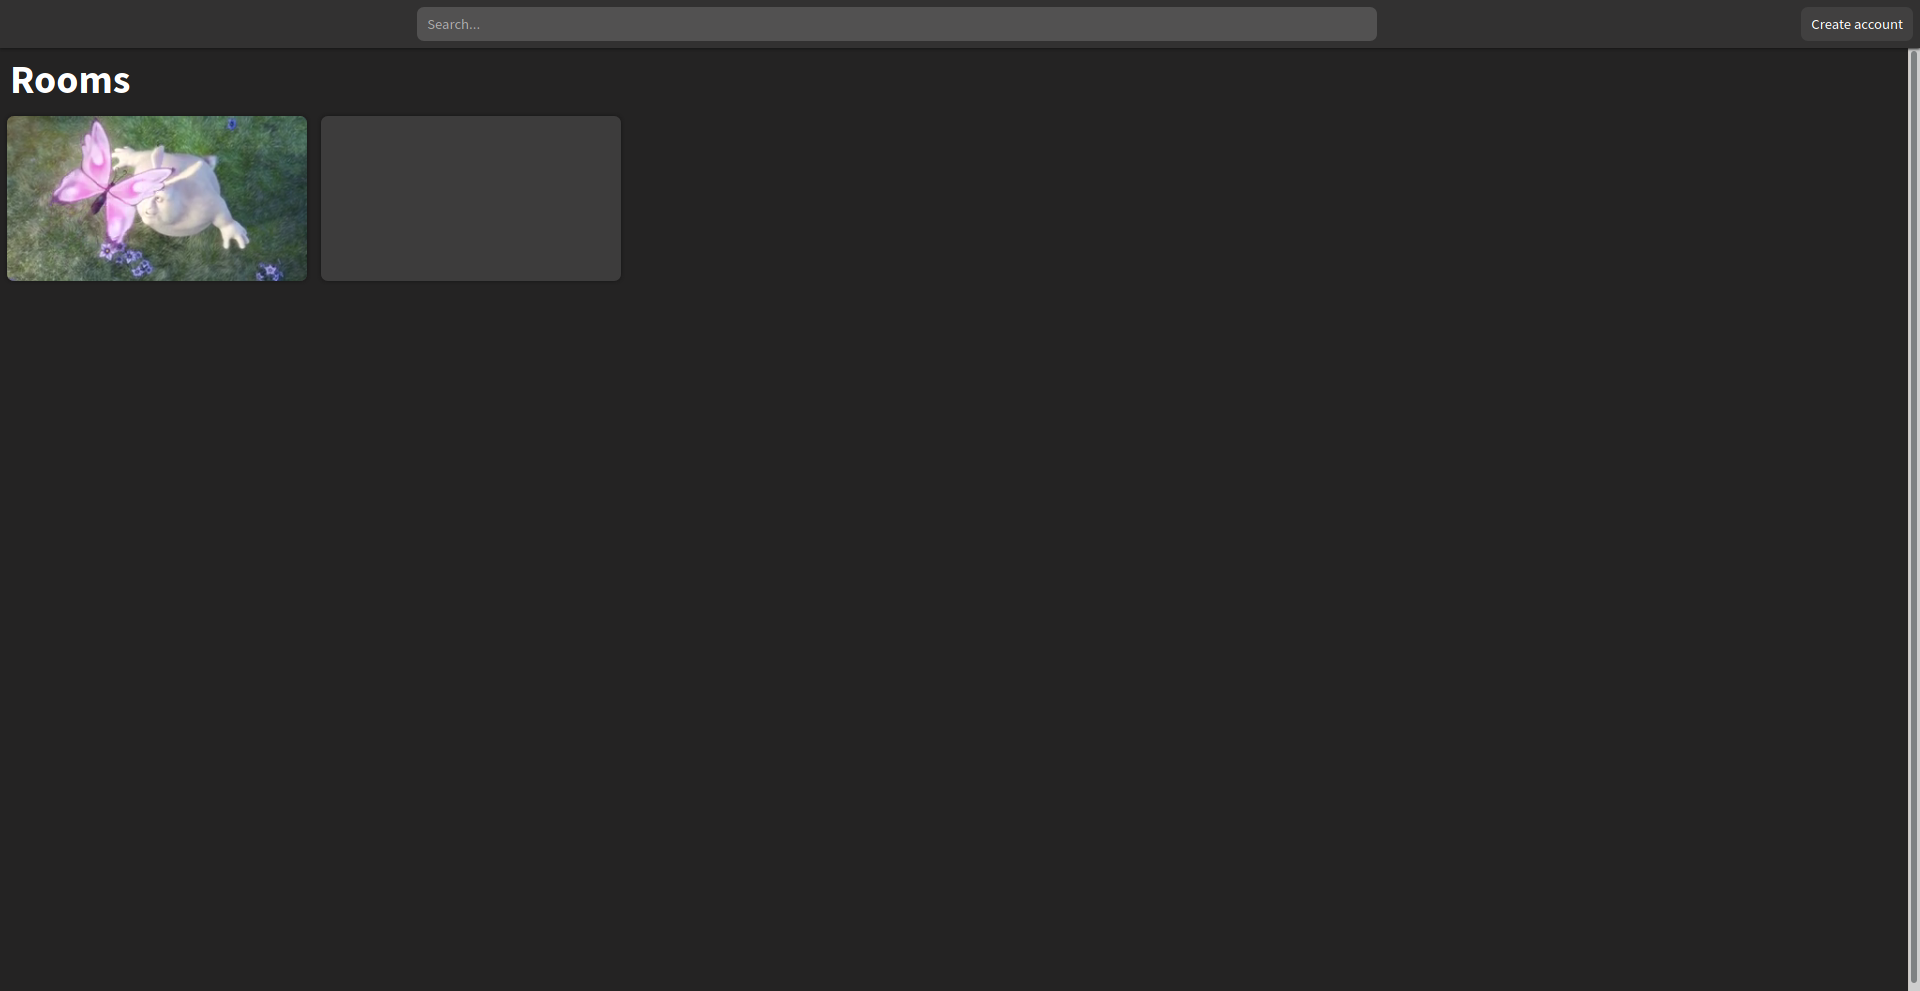
\includegraphics[scale=0.24]{main.png} 
%   \caption{Главная страница приложения}
%   \label{fig:arch:main_page}
%\end{figure}
% 
%\begin{figure}[H]
% \centering
%   
\includegraphics[scale=0.24]{room.jpg} 
%   \caption{Страница комнаты}
%   \label{fig:arch:room_page}
%\end{figure}
% 
%Основная страница содержит в себе следующий набор функциональных возможностей:
%\begin{itemize}
% \item авторизация пользователей;
% \item изменение пользовательских настроек;
% \item отображение доступных комнат;
% \item поиск комнат;
% \item предпросмотр комнат;
% \item переход на страницу комнаты.
%\end{itemize}
% 
%Станица плеера имеет следующие функции:
%\begin{itemize}
% \item проверка пароля комнаты;
% \item сохранение пароля при удачном вводе, чтобы пропустить его ввод в дальнейшем;
% \item воспроизведение видеоролика;
% \item остановка видеоролика;
% \item перемотка видеоролика;
% \item изменение громкости видеоролика;
% \item открытие видеоролика в полноэкранном режиме;
% \item отображение уведомлений о текущих действиях плеера;
% \item добавление видеоролика в список воспроизведения;
% \item добавление нескольких роликов в список воспроизведения;
% \item удаление ролика из списка воспроизведения;
% \item удаление всех роликов из списка воспроизведения;
% \item выбор следующего ролика для воспроизведения из списка воспроизведения;
% \item автоматическое включение следующего ролика из списка воспроизведения;
% \item синхронизация времени ролика между пользователями текущей комнаты;
% \item синхронизация состояния воспроизведения между пользователями текущей комнаты;
% \item синхронизация источника текущего видеоролика между пользователями текущей комнаты;
% \item отправка и получение сообщений в чате комнаты.
%\end{itemize}
% 
%\subsection{Учётная запись пользователя}
%Для работы пользователя с веб-приложением необходимо иметь учетную запись. Каждый пользователь при первом открытии страницы приложения автоматически получает учетную %запись без необходимости ввода каких-либо данных. Данная учетная запись имеет статус анонимной. Это сделано для того чтобы любой пользователь мог сразу начать %пользоваться сервисом. Пользователи с анонимной учетной записью имеют ряд ограничений:
%\begin{itemize}
% \item невозможно создать собственную комнату;
% \item невозможно сменить имя пользователя;
%\end{itemize}
% 
%Для того чтобы избавиться от ограничений пользователю необходимо создать собственную учетную запись. Для этого ему необходимо предоставить адрес электронной почты, %выбрать имя пользователя и пароль (для подтверждения пароля пользователь должен ввести его два раза). 
%В дальнейшем пользователь при посещении сайта будет сразу использовать созданную им учетную запись.
%Для сохранения пользовательской информации в рамках текущей сессии, она записывается в хранилище состояний, предоставленный JavaScript библиотекой Redux.
% 
%\subsection{Список комнат}
%Каждый пользователь имеет возможность просмотра списка комнат на главной странице. Данные для данного списка загружаются из базы данных и автоматически обновляются при %их изменении.
%Также пользователь имеет возможность производить поиск комнат, для этого имеется строка поиска в верхней части страницы.
% 
%Список комнат представлен в виде набора плиток. На данных плитках находится основная информация о данной комнате: название, защищённость паролем, а также окно %предпросмотра текущего видеоролика. 
%При нажатии на плитку комнаты пользователь перенаправляется на страницу данной комнаты. 
%
%\subsection{Комната}
%Перед тем как получить доступ к комнате происходит дополнительная проверка. 
%Если комната защищена паролем, то пользователь сначала попадает на страницу с формой для ввода пароля. 
%В случае ввода неправильного пароля пользователь получает уведомление об ошибке и ему предлагается ввести пароля снова. 
%При вводе верного пароля, он сохраняется в локальном хранилище браузера для повторного использования и пользователь получает доступ к комнате. 
%
%\subsection{Варианты использования}
%Далее будут рассмотрены основные варианты использования разработанного веб-приложения.
%
%\subsubsection{ВИ Создание учётной записи}~\par
%\label{use:reg}
%Описание ВИ: Пользователь имеет возможность при желании создать личную учётную запись.
% 
%Предусловия основного потока действий нет.
% 
%Основной поток действий:
%\begin{itemize}
%   \item пользователь нажимает кнопку "Create account";
%   \item пользователь вводит электронную почту, имя пользователя, пароль и подтверждение пароля.
%\end{itemize}
% 
%Ограничения: различные ограничения, установленные провайдером аутентификации Firebase.
% 
%\subsubsection{ВИ Использование своей учётной записи}~\par
%Описание ВИ: Пользователь имеет возможность использовать личную учётную запись.
% 
%Предусловия основного потока действий: у пользователя имеется учётная запись см.~\ref{use:reg}.
% 
%Основной поток действий:
%\begin{itemize}
%   \item пользователь нажимает кнопку "Create account";
%   \item пользователь нажимает кнопку "Existing user";
%   \item пользователь вводит электронную почту и пароль.
%\end{itemize}
% 
%Ограничения: различные ограничения, установленные провайдером аутентификации Firebase.
%
%\subsubsection{ВИ Создание комнаты}~\par
%\label{use:roomcreate}
%Описание ВИ: Пользователь имеет возможность создать комнату для совместного просмотра.
% 
%Предусловия основного потока действий: пользователь должен быть авторизован.
% 
%Основной поток действий:
%\begin{itemize}
%   \item пользователь нажимает кнопку "Create";
%   \item пользователь вводит название комнаты и пароль;
%   \item клиент получает список комнат и обновляет интерфейс.
%\end{itemize}
% 
%Ограничения: имя комнаты должно быть непустой строкой.
% 
%\subsubsection{ВИ Поиск комнаты}~\par
%Описание ВИ: Пользователь имеет возможность искать комнату по её имени для совместного просмотра.
% 
%Предусловия основного потока действий: Комната существует. Для создания комнаты см.~\ref{use:roomcreate}.
% 
%Основной поток действий:
%\begin{itemize}
%   \item пользователь начинает писать название комнаты;
%   \item при изменении текста в строке поиска система делает поиск по имени комнаты;
%   \item клиент получает список комнат и обновляет свой интерфейс.
%\end{itemize}
% 
%Ограничения: имя комнаты должно быть непустой строкой.
%
%\subsubsection{ВИ Подключение к комнате}~\par
%\label{use:join}
%Описание ВИ: Пользователь имеет возможность присоединиться к комнате для совместного просмотра.
% 
%Предусловия основного потока действий: комната должна существовать см.~\ref{use:roomcreate}.
% 
%Основной поток действий:
%\begin{itemize}
%   \item пользователь нажимает кнопку плитку комнаты из списка;
%   \item пользователь перенаправляется на страницу комнаты.
%\end{itemize}
% 
%Ограничения: при наличии у комнаты пароля пользователь должен ввести его, для подключения.
% 
%\subsubsection{ВИ Управление видеоплеером}~\par
%Описание ВИ: Пользователь имеет возможность управлять видеоплеером комнаты во время совместного просмотра.
% 
%Предусловия основного потока действий: комната должна существовать см.~\ref{use:roomcreate}, Пользователь присоединен к комнате см.~\ref{use:join}.
% 
%Основной поток действий:
%\begin{itemize}
%   \item Пользователь имеет следующие опций для управления плеером: запуск и остановка воспроизведения видео, перемотка, настройка громкости, открытие полноэкранного %режима.
%\end{itemize}
% 
%Ограничения: Для взаимодействия с плеером должно быть выбрано видео для воспроизведения см.~\ref{use:addvideo}.
% 
%\subsubsection{ВИ Добавление видео по ссылке}~\par
%\label{use:addvideo}
%Описание ВИ: Пользователь имеет возможность добавить видео в список воспроизведения комнаты для совместного просмотра.
% 
%Предусловия основного потока действий: комната должна существовать см.~\ref{use:roomcreate}, Пользователь присоединен к комнате см.~\ref{use:join}.
% 
%Основной поток действий:
%\begin{itemize}
%   \item пользователь открывает меню списка воспроизведения;
%   \item пользователь нажимает кнопку "Add";
%   \item пользователь вводит ссылку на ролик в строку поиска;
%   \item клиент получает список видео и обновляет интерфейс;
%   \item пользователь нажимает кнопку "Add" у нужного видеоролика.
%\end{itemize}
% 
%Ограничения: ссылка должна поддерживаться приложением.
% 
%\subsubsection{ВИ Удаление видео из списка воспроизведения}~\par
%Описание ВИ: Пользователь имеет возможность удалить видео в список воспроизведения комнаты для совместного просмотра.
% 
%Предусловия основного потока действий: комната должна существовать см.~\ref{use:roomcreate}, Пользователь присоединен к комнате см.~\ref{use:join}, в списке %воспроизведения должны быть видеоролики см.~\ref{use:addvideo}.
% 
%Основной поток действий:
%\begin{itemize}
%   \item пользователь открывает меню списка воспроизведения;
%   \item пользователь нажимает кнопку "крестик" у необходимого видеоролика.
%\end{itemize}
% 
%Альтернативный поток действий:
%\begin{itemize}
%   \item пользователь открывает меню списка воспроизведения;
%   \item пользователь нажимает кнопку "Reset".
%\end{itemize}
% 
%Ограничений нет.
% 
%\subsubsection{ВИ Использование чата}~\par
%Описание ВИ: Пользователь имеет возможность общаться с другими пользователями, используя текстовый чат.
% 
%Предусловия основного потока действий: комната должна существовать см.~\ref{use:roomcreate}, Пользователь присоединен к комнате см.~\ref{use:join}.
% 
%Основной поток действий:
%\begin{itemize}
%   \item пользователь открывает текстовый чат;
%   \item пользователь вводит сообщение в текстовое поле;
%   \item пользователь нажимает кнопку "Send" или клавишу Enter.
%\end{itemize}
% 
%Ограничения: сообщение должно быть непустой строкой.
%
%\subsection{Тестирование приложения}
% 
%Для проведения тестирования веб-приложения использовалось ПО из проекта Selenium. 
%В рамках данного проекта разработан набор различных программ, которые помогают автоматизировать процесс тестирования веб-приложений. 
%Для данного проекта использовался Selenium WebDriver - универсальный интерфейс для взаимодействия с драйвером браузера, веб-браузер Firefox и драйвер geckodriver. 
%Для проведения тестов использовалась библиотека для языка Python и расширение для браузера Firefox~--- Selenium IDE.
% 
%Также было проведено ручное тестирование механизма синхронизации, так как при помощи Selenium их протестировать затруднительно. 
%В рамках ручного тестирования было проведено дымовое тестирование возможностей видеоплеера и механизмов синхронизации.
%